\section{Empirical Comparison}
\label{sec:empirical_comparison}

We now provide a detailed empirical comparison for the advantage and
disadvantage of the data transfer methods presented in
Section~\ref{sec:data_transfer_methods}.
Our experimental setup is composed of an Intel Core i7 2600 processor
and an NVIDIA GeForce GTX~480 graphics card.
We use the Linux kernel v2.6.42 and Gdev~\cite{Kato_ATC12} as the
underlying OS and GPGPU runtime/driver software respectively.
This set of open-source platforms allows our implementations of the
investigated data transfer methods.

The test programs are written in CUDA~\cite{NVIDIA_CUDA} and are compiled
using the NVIDIA CUDA Compiler (NVCC) v4.2~\cite{NVIDIA_NVCC}.
Note that Gdev is compatible with this binary compiler toolkit.
We exclude compute kernels and focus on data transfer functions in this
empirical comparison.
While the test programs uniformly use the same CUDA API functions, we
provide different internal implementations according to the target data
transfer methods.

Data streams between the host and the device memory are provided by a
single GPU context.
Performance interference among multiple GPU contexts is outside the
scope of this paper.
We evaluate the data transfer performances of both real-time and normal
tasks.
For the scheduling policies of the Linux kernel, we use
\texttt{SCHED\_FIFO} for real-time tasks while \texttt{SCHED\_OTHER} for
normal tasks, where the real-time tasks are always prioritized over the
normal tasks.
The real-time capability relies on the default performance of the
real-time scheduling class supported by the Linux kernel.
We believe that this setup is sufficient for our experiments given that
we execute at most one real-time task in the system while multiple data
streams may be produced by this task.
Overall the scheduling performance issues are outside the scope of this
paper.

Henceforth we use the following labels to denote the investigated data
transfer methods respectively:
\begin{itemize}
 \item \textbf{DMA} denotes the standard DMA method presented in
       Section~\ref{sec:dma}.
 \item \textbf{IORW} denotes the memory-mapped read and write method
       presented in Section~\ref{sec:iorw}.
 \item \textbf{MEMWND} denotes the memory-window read and write method
       presented in Section~\ref{sec:memwnd}.
 \item \textbf{HUB} denotes the microcontroller-based data transfer
       method presented in Section~\ref{sec:micro}, particularly using a
       \textit{hub} microcontroller designed to broadcast among the
       actual microcontrollers of graphics processing clusters (GPCs),
       \textit{i.e.}, CUDA core clusters.
 \item \textbf{GPC} denotes the microcontroller-based data transfer
       method presented in Section~\ref{sec:micro}, particularly using a
       single GPC microcontroller.
 \item \textbf{GPC4} denotes the microcontroller-based data transfer
       method presented in Section~\ref{sec:micro}, particularly using
       four different GPC microcontrollers in parallel.
       Note that the NVIDIA Fermi architecture~\cite{NVIDIA_Fermi}
       provides four GPCs and their microcontrollers can perform
       individually.
       Therefore we can split the data transfer into four pieces and
       make the four microcontrollers work in parallel.
\end{itemize}

\subsection{Basic Performance}

\begin{figure}[!t]
 \begin{center}
  \subfigure[Host to Device]{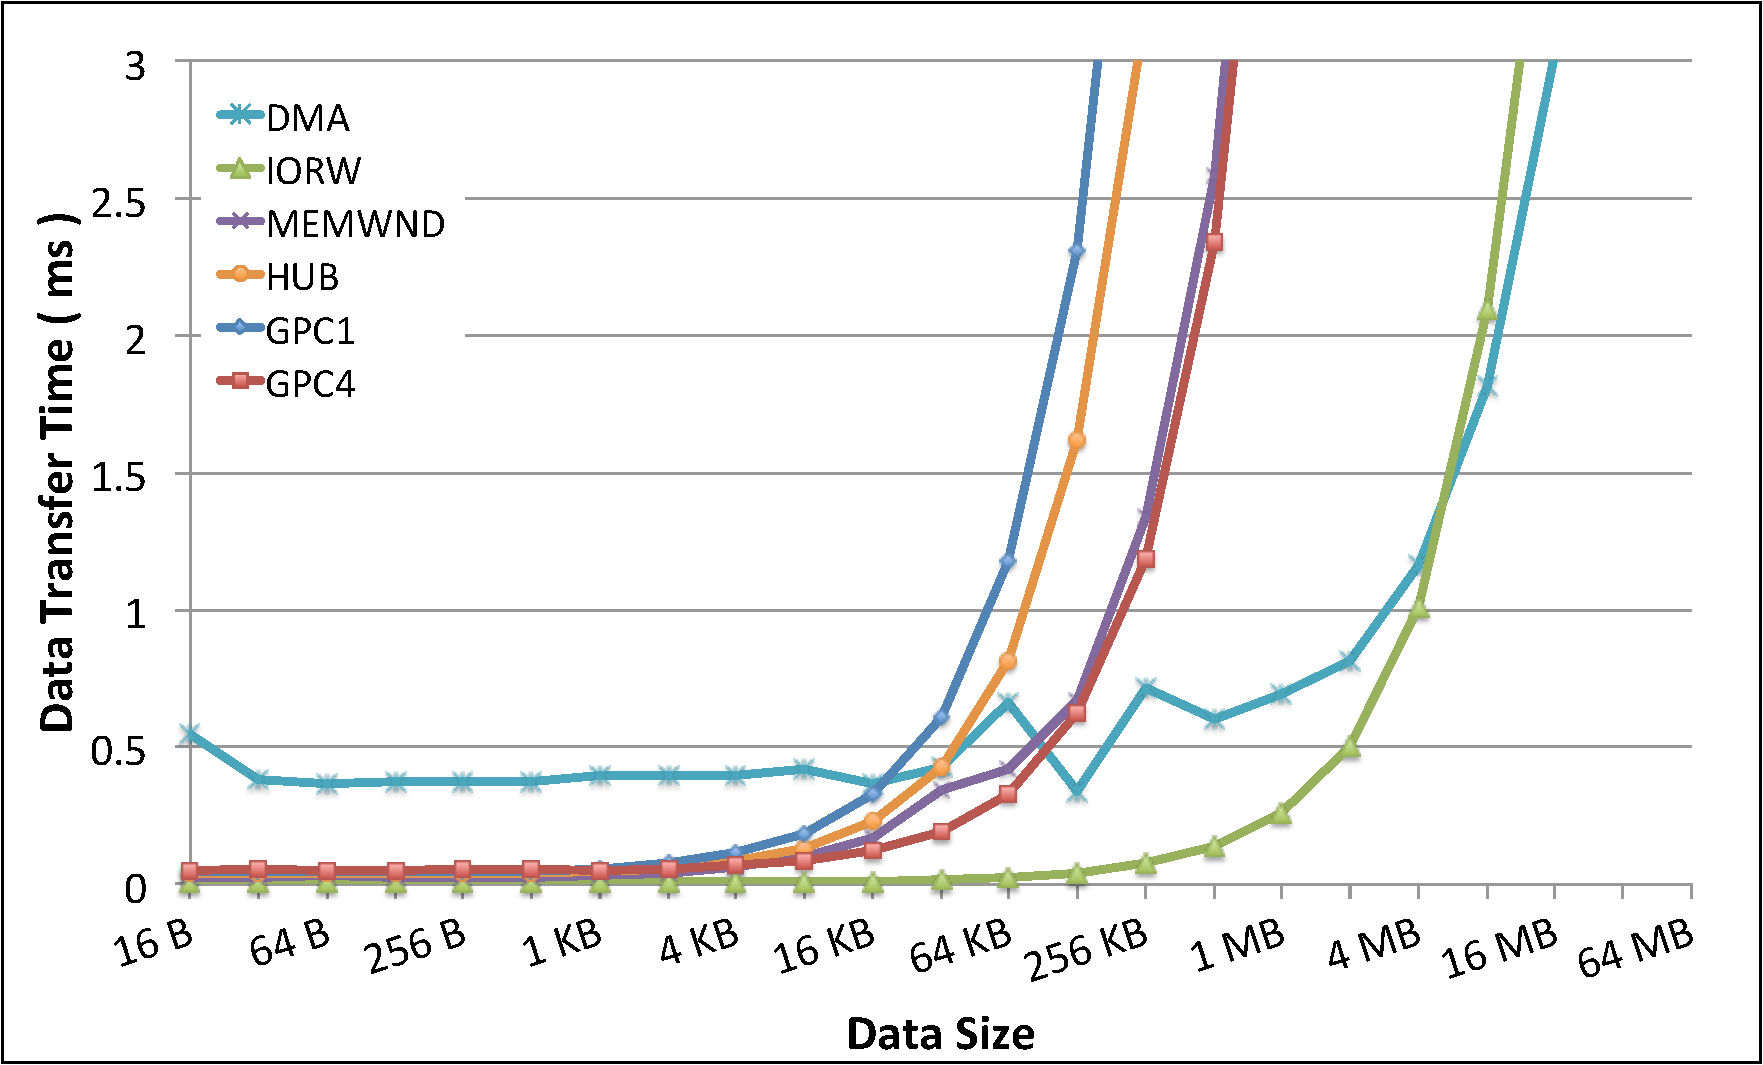
\includegraphics[width=0.34\textwidth]{figure/Graph/realtask/Memcpy_rtask_normal_HtoD.pdf}}\\
  \subfigure[Device to Host]{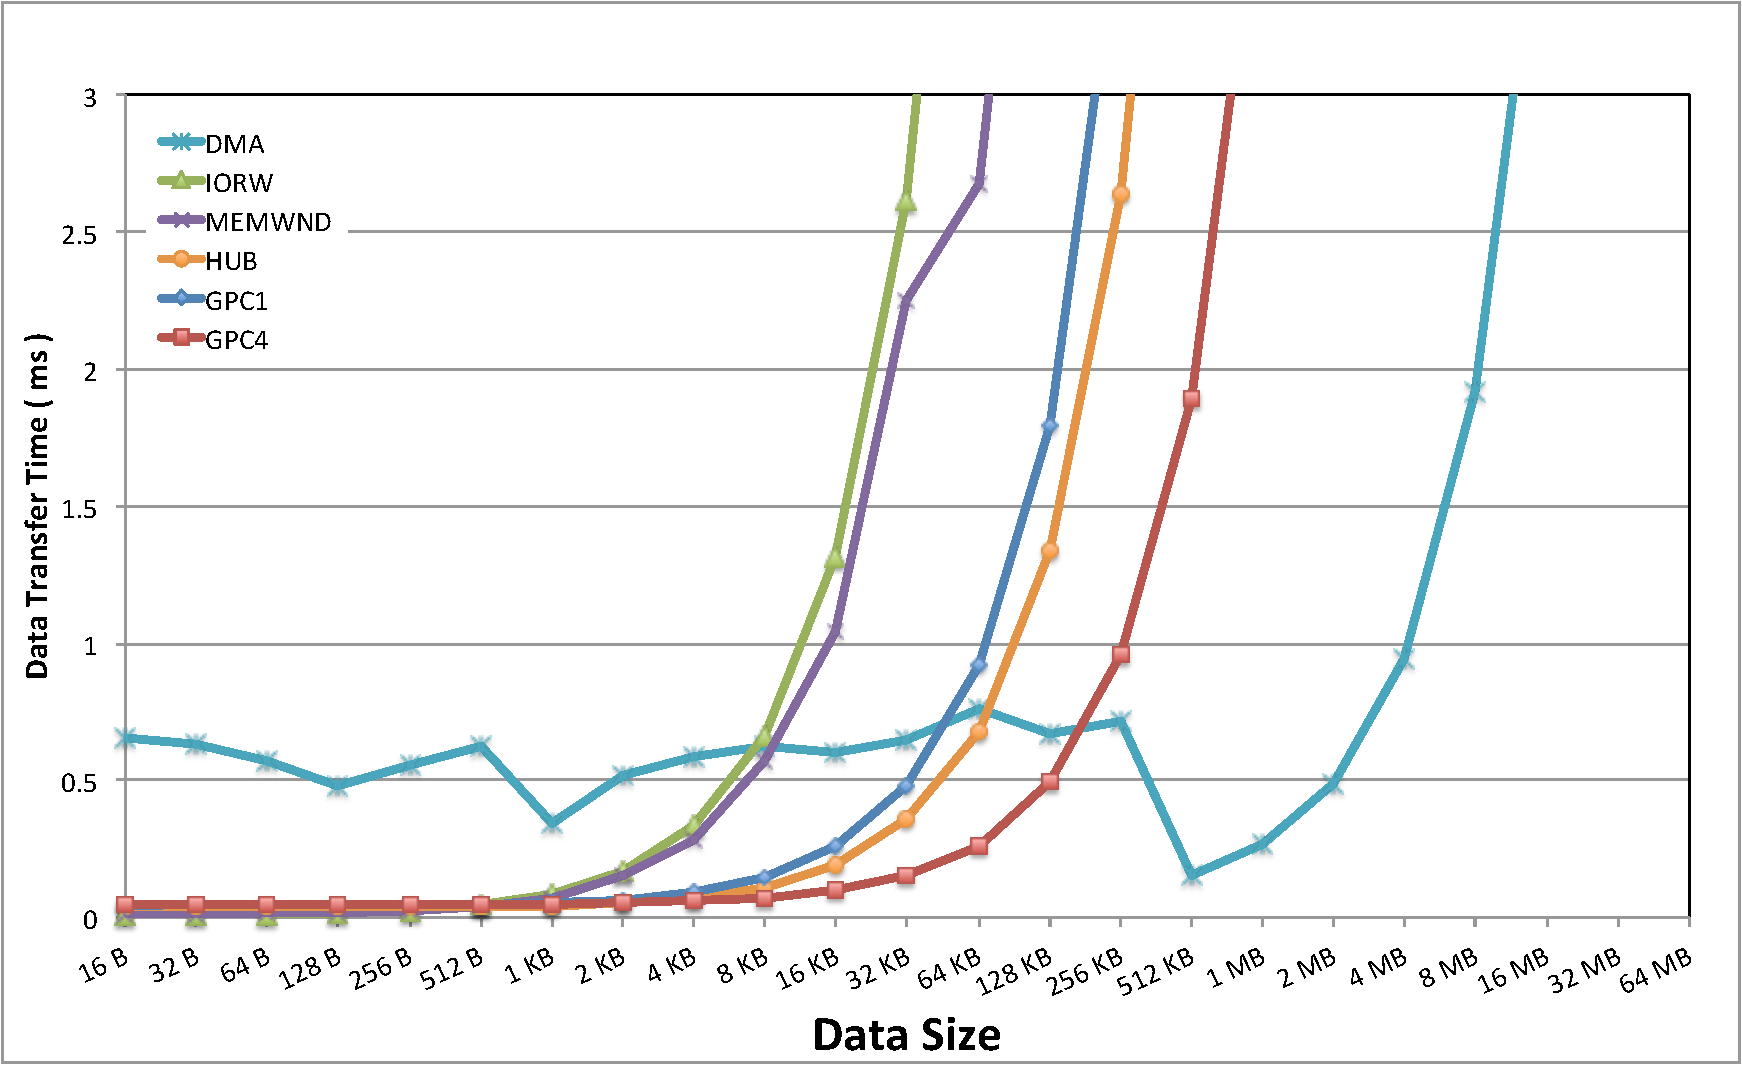
\includegraphics[width=0.34\textwidth]{figure/Graph/realtask/Memcpy_rtask_normal_DtoH.pdf}}
  \caption{Average performance of each data transfer method with a
  real-time task.}
  \label{fig:average_realtime}
 \end{center}
 \vspace{0.5em}
 \begin{center}
  \subfigure[Host to Device]{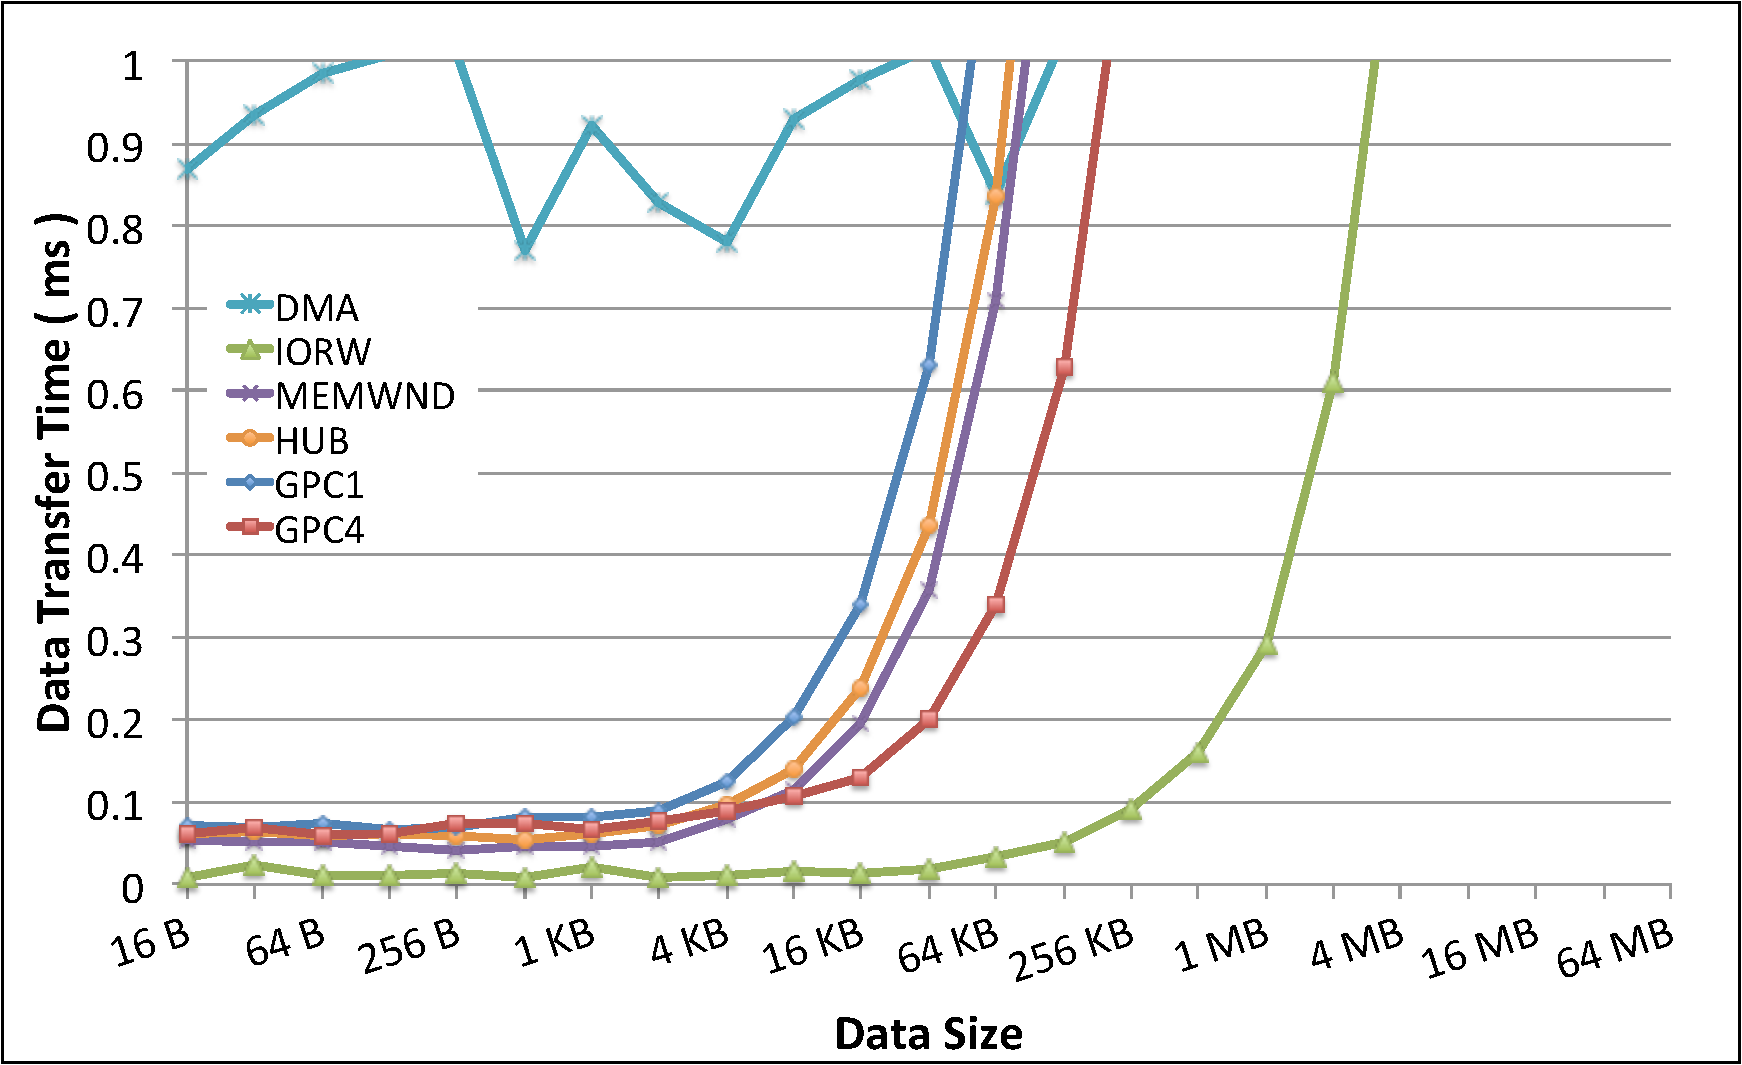
\includegraphics[width=0.34\textwidth]{figure/Graph/realtask/Memcpy_rtask_normal_HtoD_worst.pdf}}\\
  \subfigure[Device to Host]{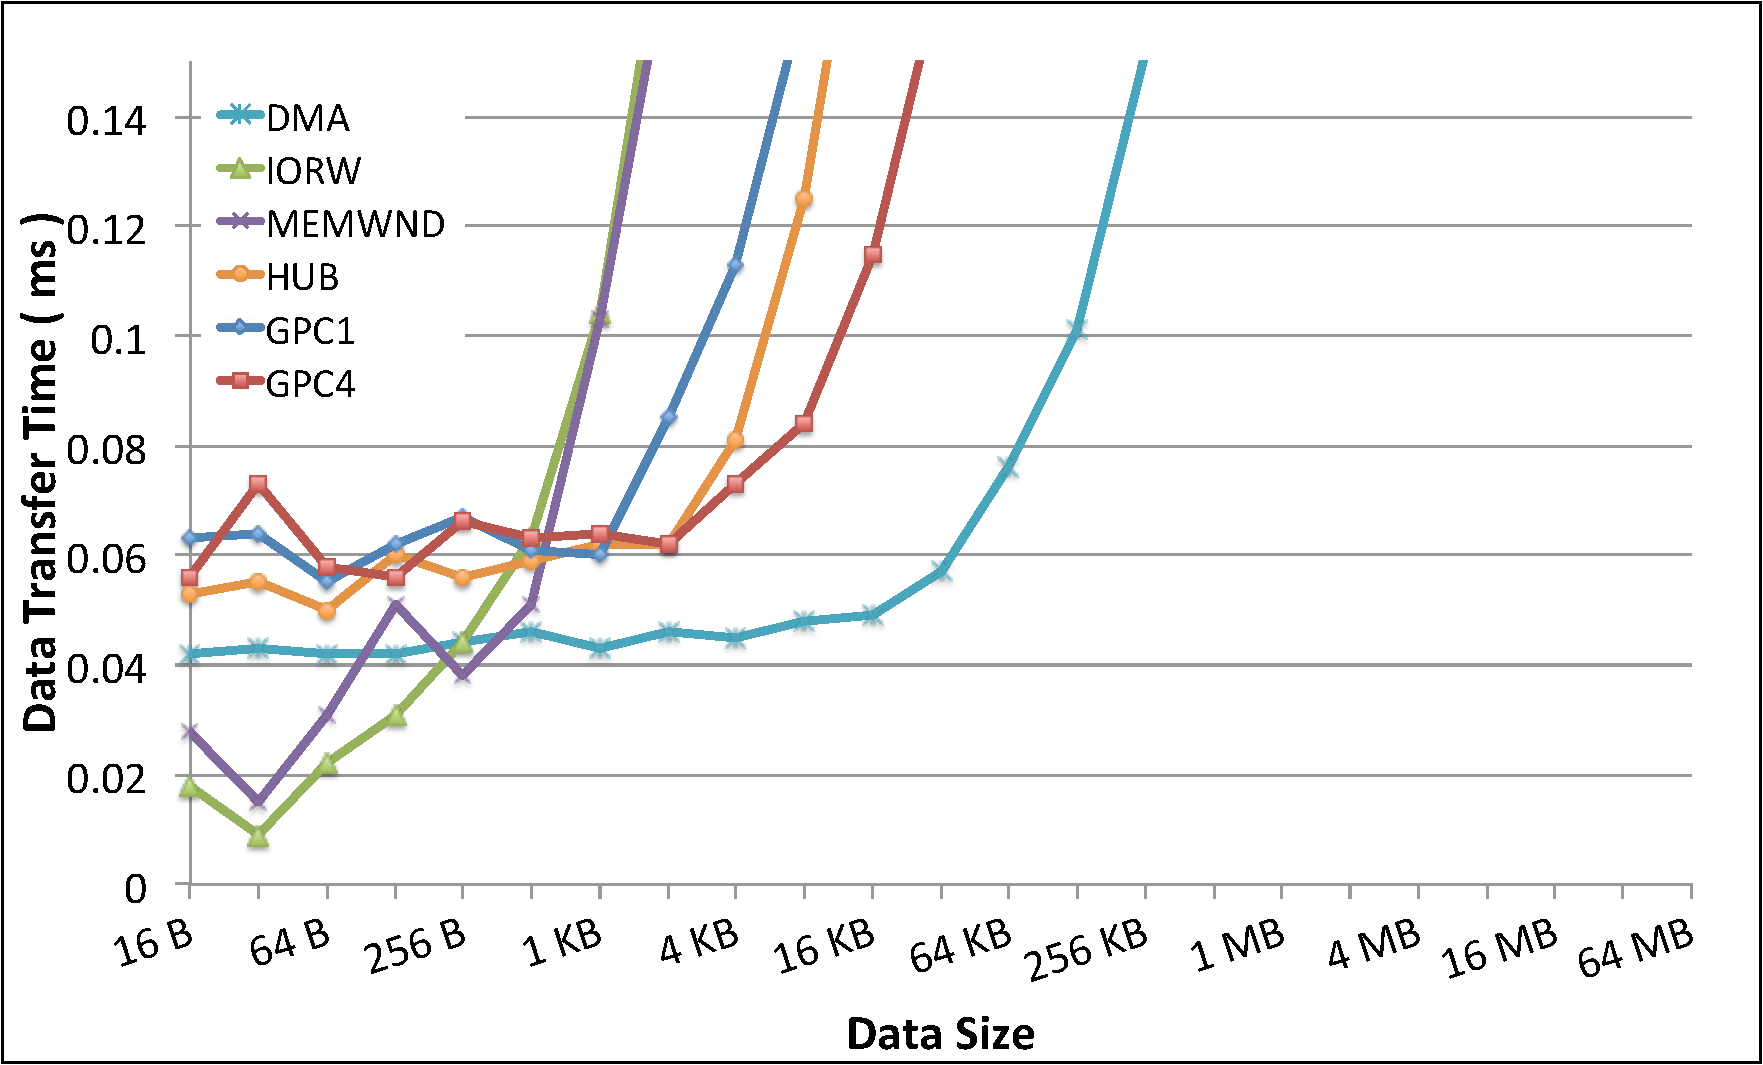
\includegraphics[width=0.34\textwidth]{figure/Graph/realtask/Memcpy_rtask_normal_DtoH_worst.pdf}}
  \caption{Worst-case performance of each data transfer method with a
  real-time task.}
  \label{fig:worst_realtime}
 \end{center}
\end{figure}

Figure~\ref{fig:average_realtime} shows the average performance of each
data transfer method when a real-time task runs alone.
Even with this most straightforward setup, there are several interesting
observations.
Performance characteristics of the host-to-device and the device-to-host
communications are not identical at all.
In particular, the performance of standard DMA exhibits a 10x difference
between the two directions of communications.
We believe that this is attributed to hardware capabilities that are not
well documented to the public.
We also find that the performances of different methods are quite
diverse but a combination of \textsf{DMA} and \textsf{IORW} can derive
the best performance.
For small data, \textsf{IORW} is preferred while \textsf{DMA} is the
best performer for large data.
The other methods are almost always inferior to either of \textsf{DMA}
or \textsf{IORW}.
The most significant finding is that \textsf{IORW} becomes very slow for
the device-to-host direction.
This is due to a design specification of the GPU.
It is designed so that the GPU can read data fast from the host computer
but compromise write access performance.
Another interesting observation is that using multiple GPC
microcontrollers to parallelize the data transfer is less effective than
a single GPC or HUB controller when the data size is small.

Figure~\ref{fig:worst_realtime} shows the worst-case performance in
the same setup as the above experiment.
It is important to note that we acquire almost the same results as those
shown in Figure~\ref{fig:average_realtime}, though there is
some degradation in the performance of \textsf{DMA} for the
host-to-device direction.
These comparisons lead to some conclusion that we may optimize the data
transfer performance by switching between \textsf{DMA} and \textsf{IORW}
at an appropriate boundary.

We omit the results of normal tasks in this setup, because they are
almost equal to those of real-time tasks shown above.
However, real-time and normal tasks behave in a very different manner in
the presence of competing workload.
This will be discussed in the next subsection.

\begin{comment}
\begin{figure}[!t]
 \begin{center}
  \subfigure[Host to Device]{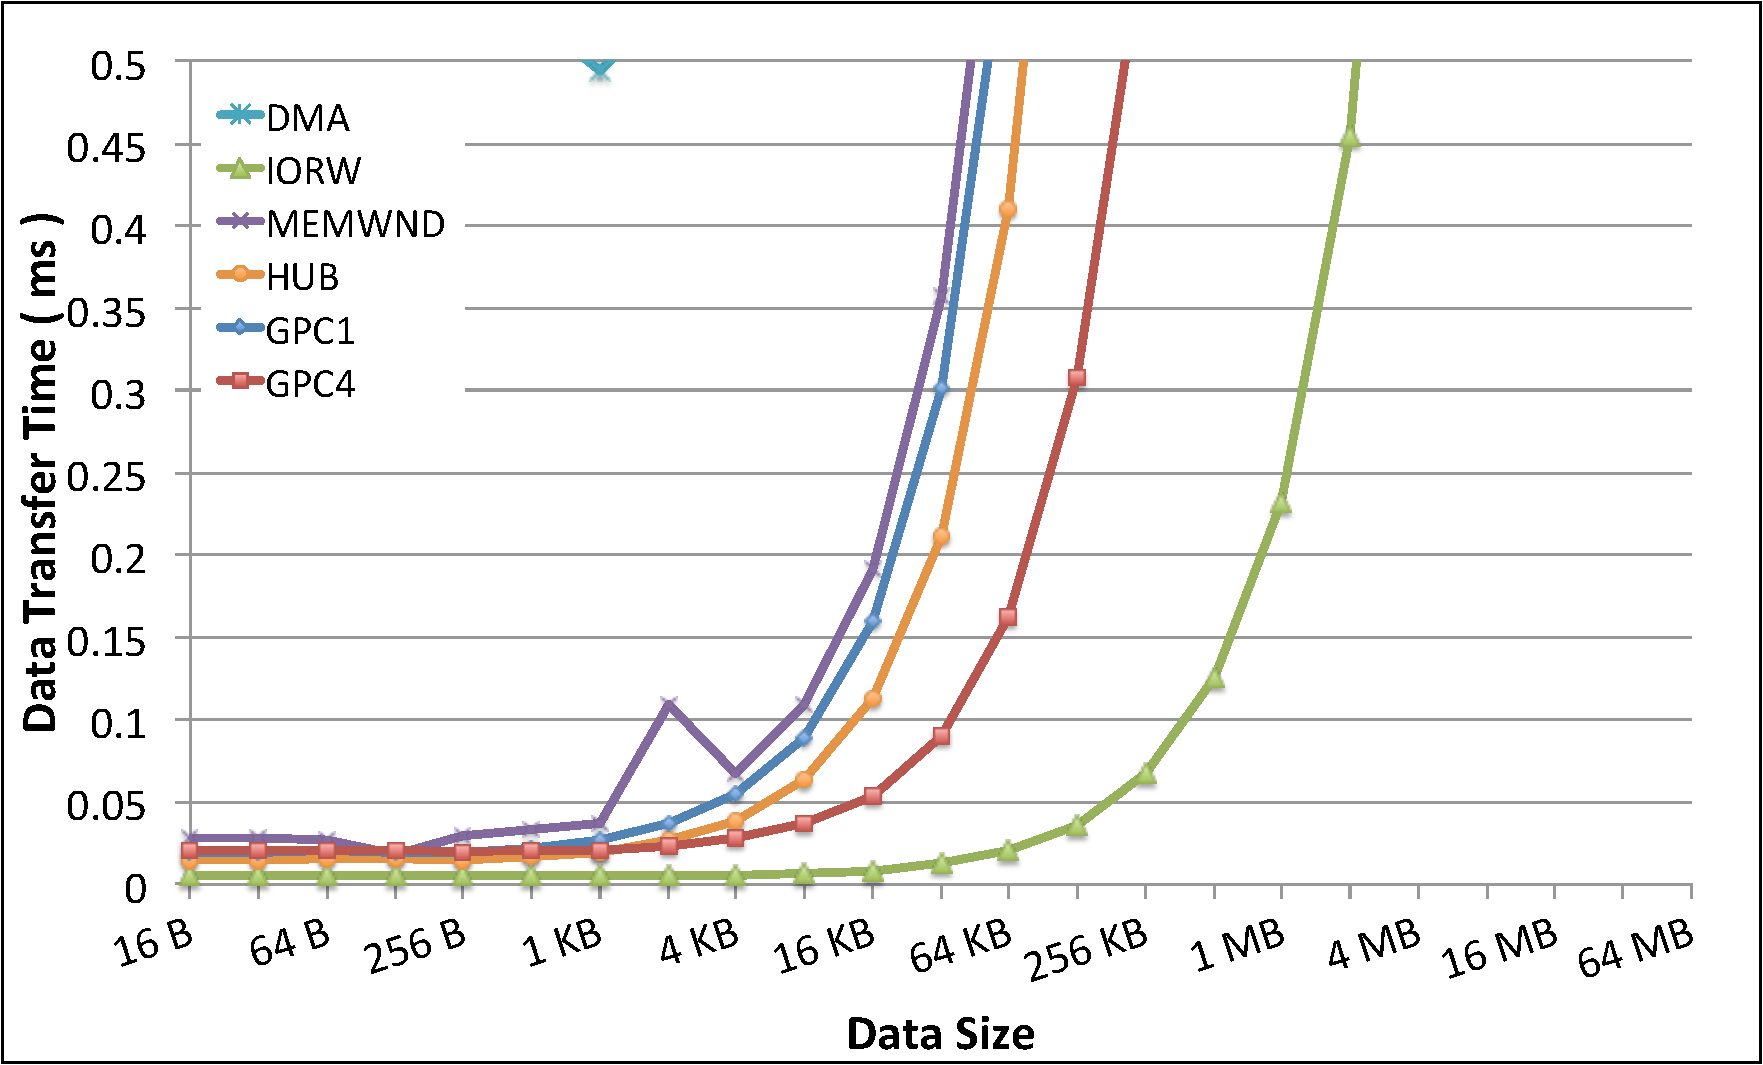
\includegraphics[width=0.34\textwidth]{figure/Graph/not_realtask/Memcpy_normal_HtoD.pdf}}\\
  \subfigure[Device to Host]{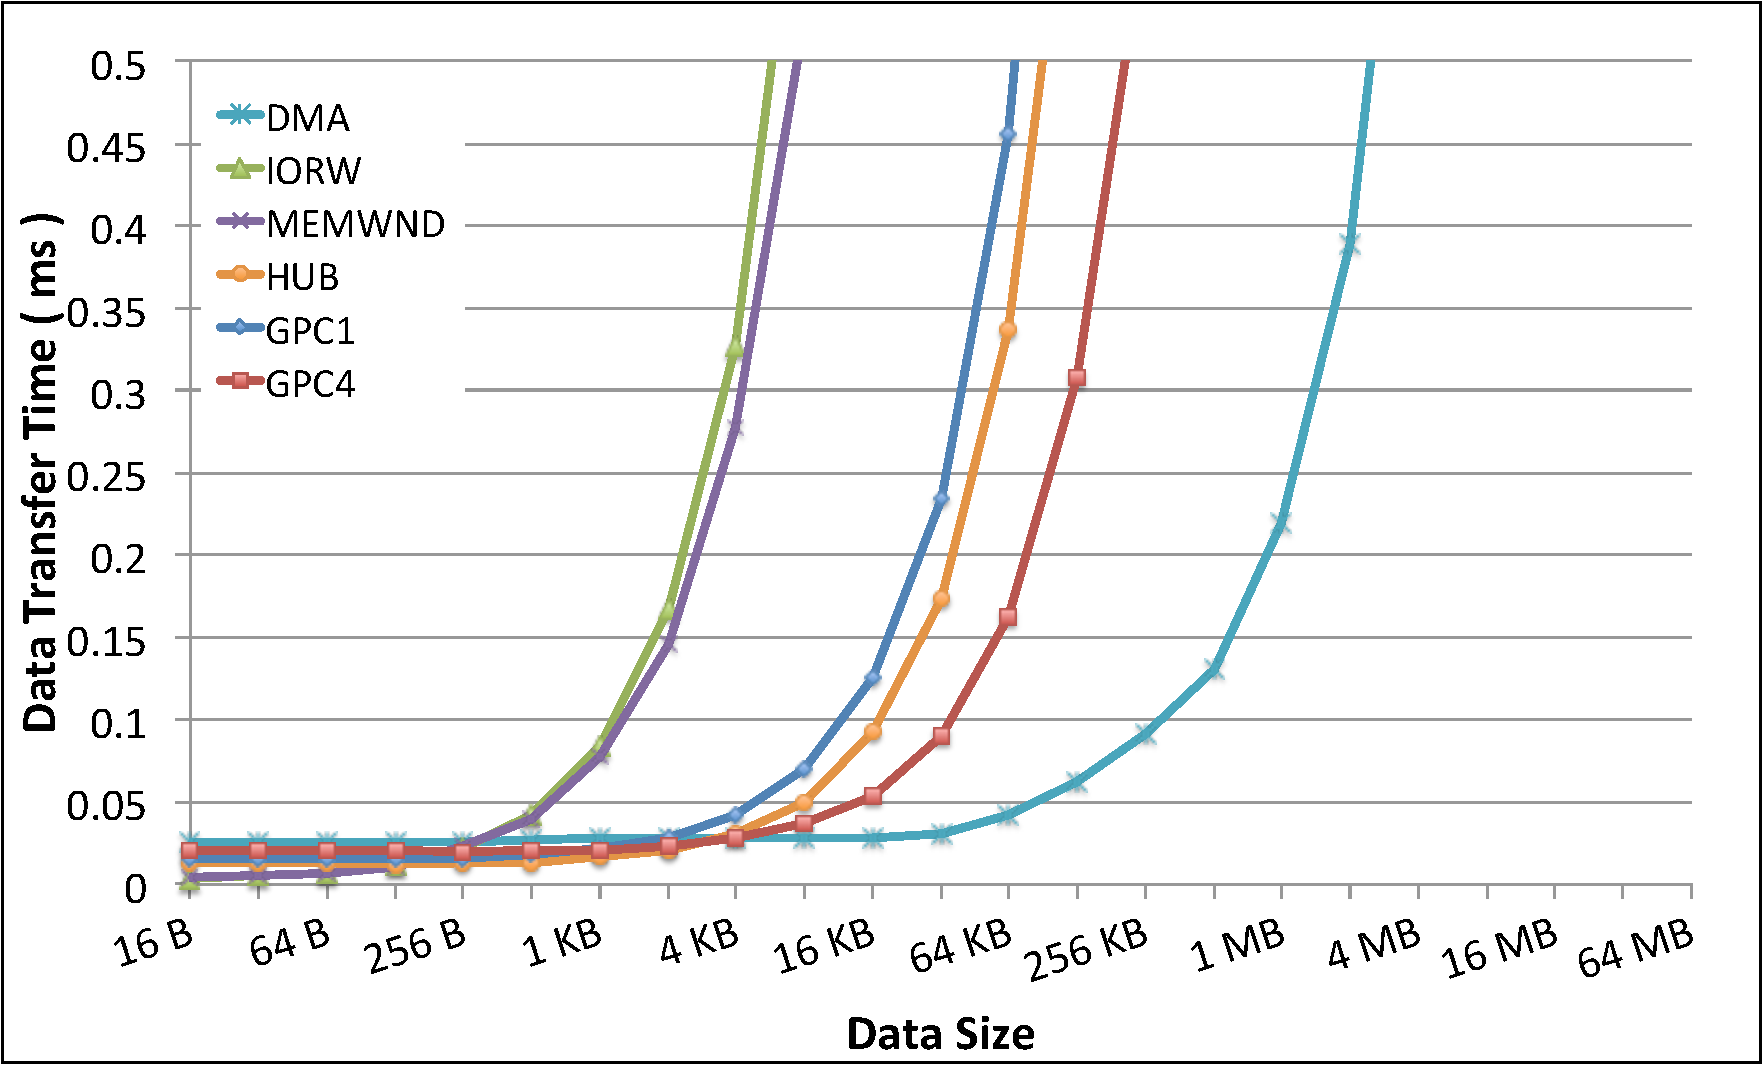
\includegraphics[width=0.34\textwidth]{figure/Graph/not_realtask/Memcpy_normal_DtoH.pdf}}
  \caption{Average performance of each data transfer method with a
  normal task.}
  \label{fig:average_normal}
 \end{center}
 \vspace{0.5em}
 \begin{center}
  \subfigure[Host to Device]{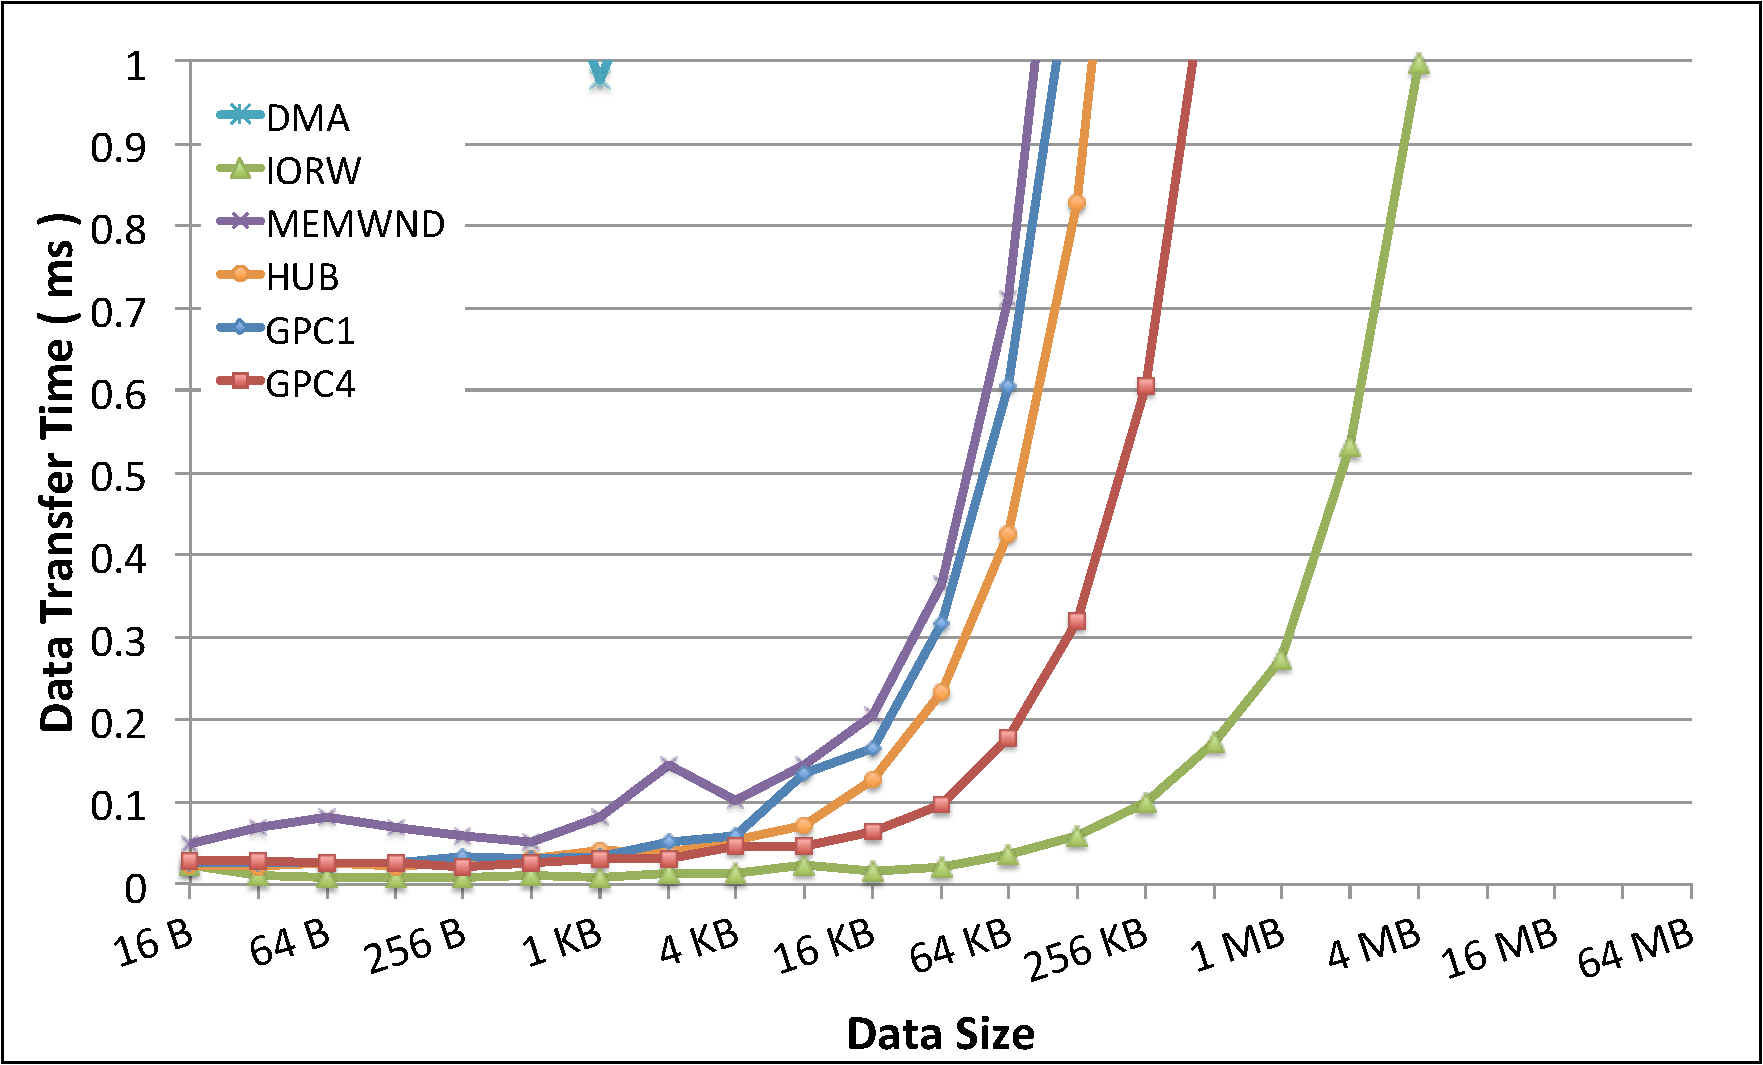
\includegraphics[width=0.34\textwidth]{figure/Graph/not_realtask/Memcpy_normal_HtoD_worst.pdf}}\\
  \subfigure[Device to Host]{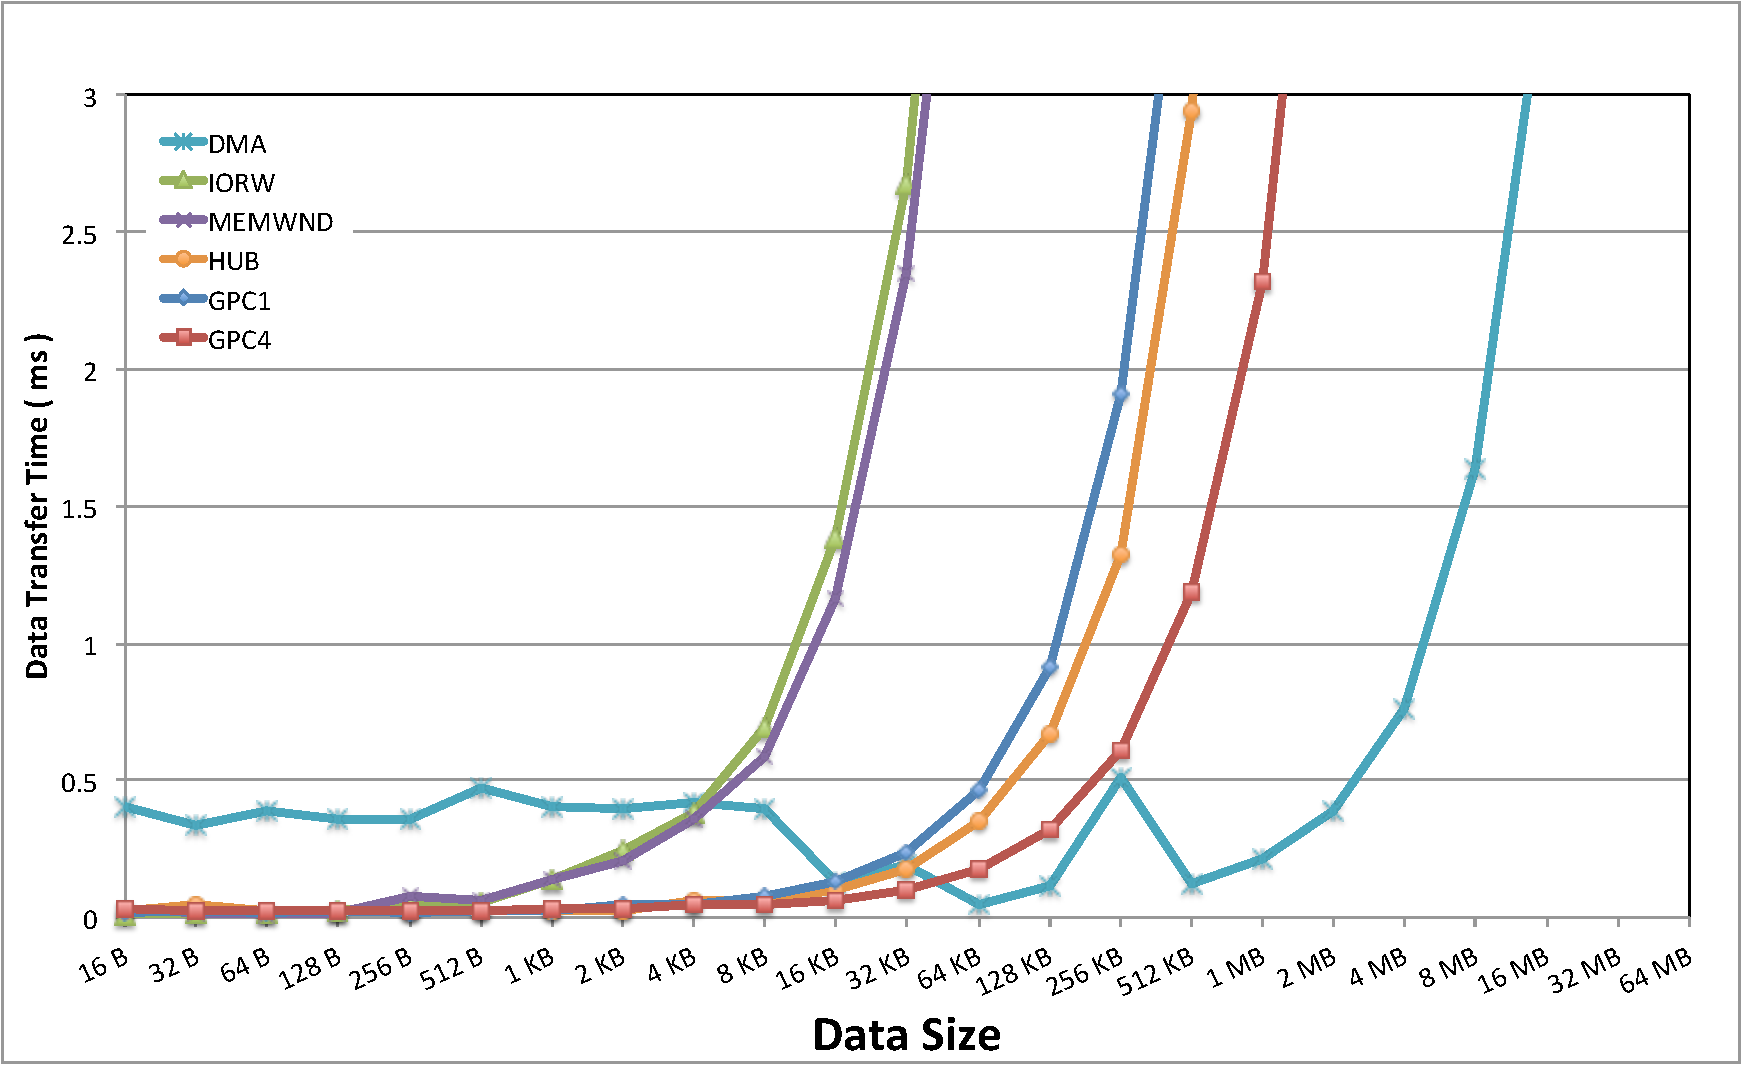
\includegraphics[width=0.34\textwidth]{figure/Graph/not_realtask/Memcpy_normal_DtoH_worst.pdf}}
  \caption{Worst-case performance of each data transfer methods with a
  normal task.}
  \label{fig:worst_normal}
 \end{center}
\end{figure}

Figure~\ref{fig:average_normal}~and~\ref{fig:worst_normal} show the
average and the worst-case performance of a normal in the same setup as
the above experiments.
\end{comment}

\subsection{Interfered Performance}

\begin{figure}[!t]
 \begin{center}
  \subfigure[Host to Device]{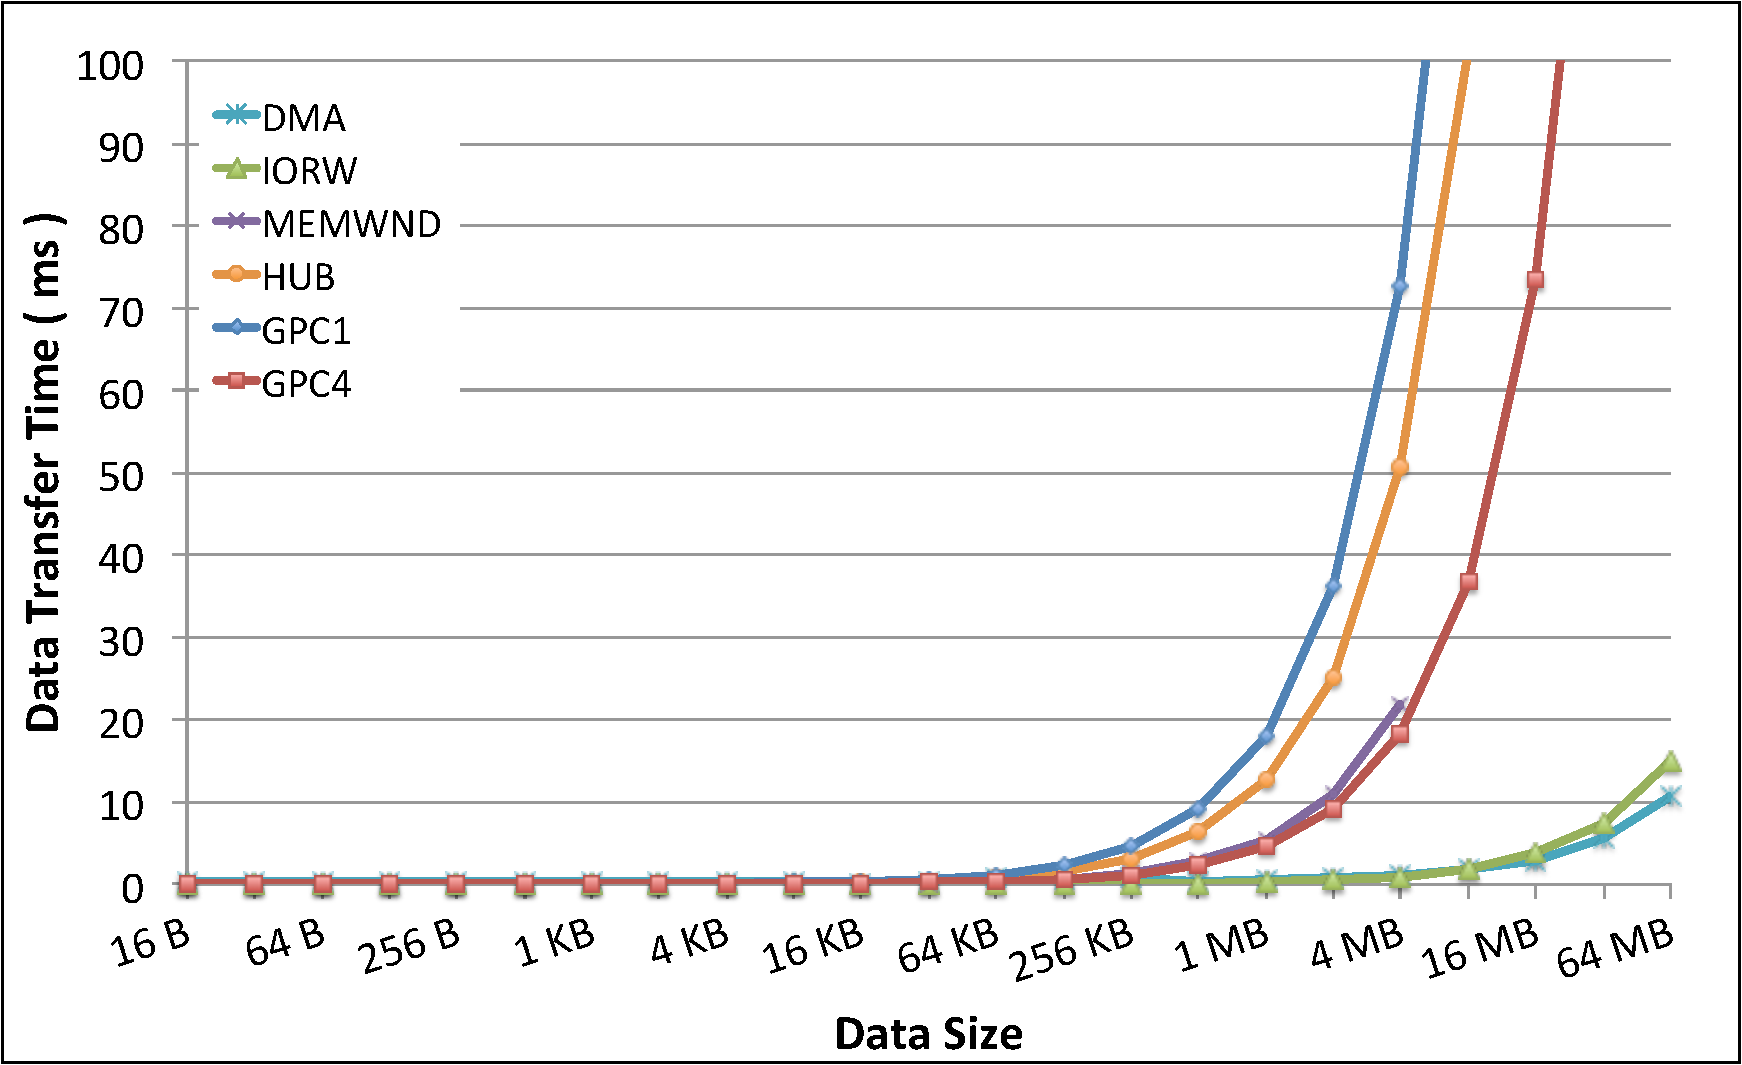
\includegraphics[width=0.34\textwidth]{figure/Graph/realtask/Memcpy_rtask_cpuload_HtoD.pdf}}\\
  \subfigure[Device to Host]{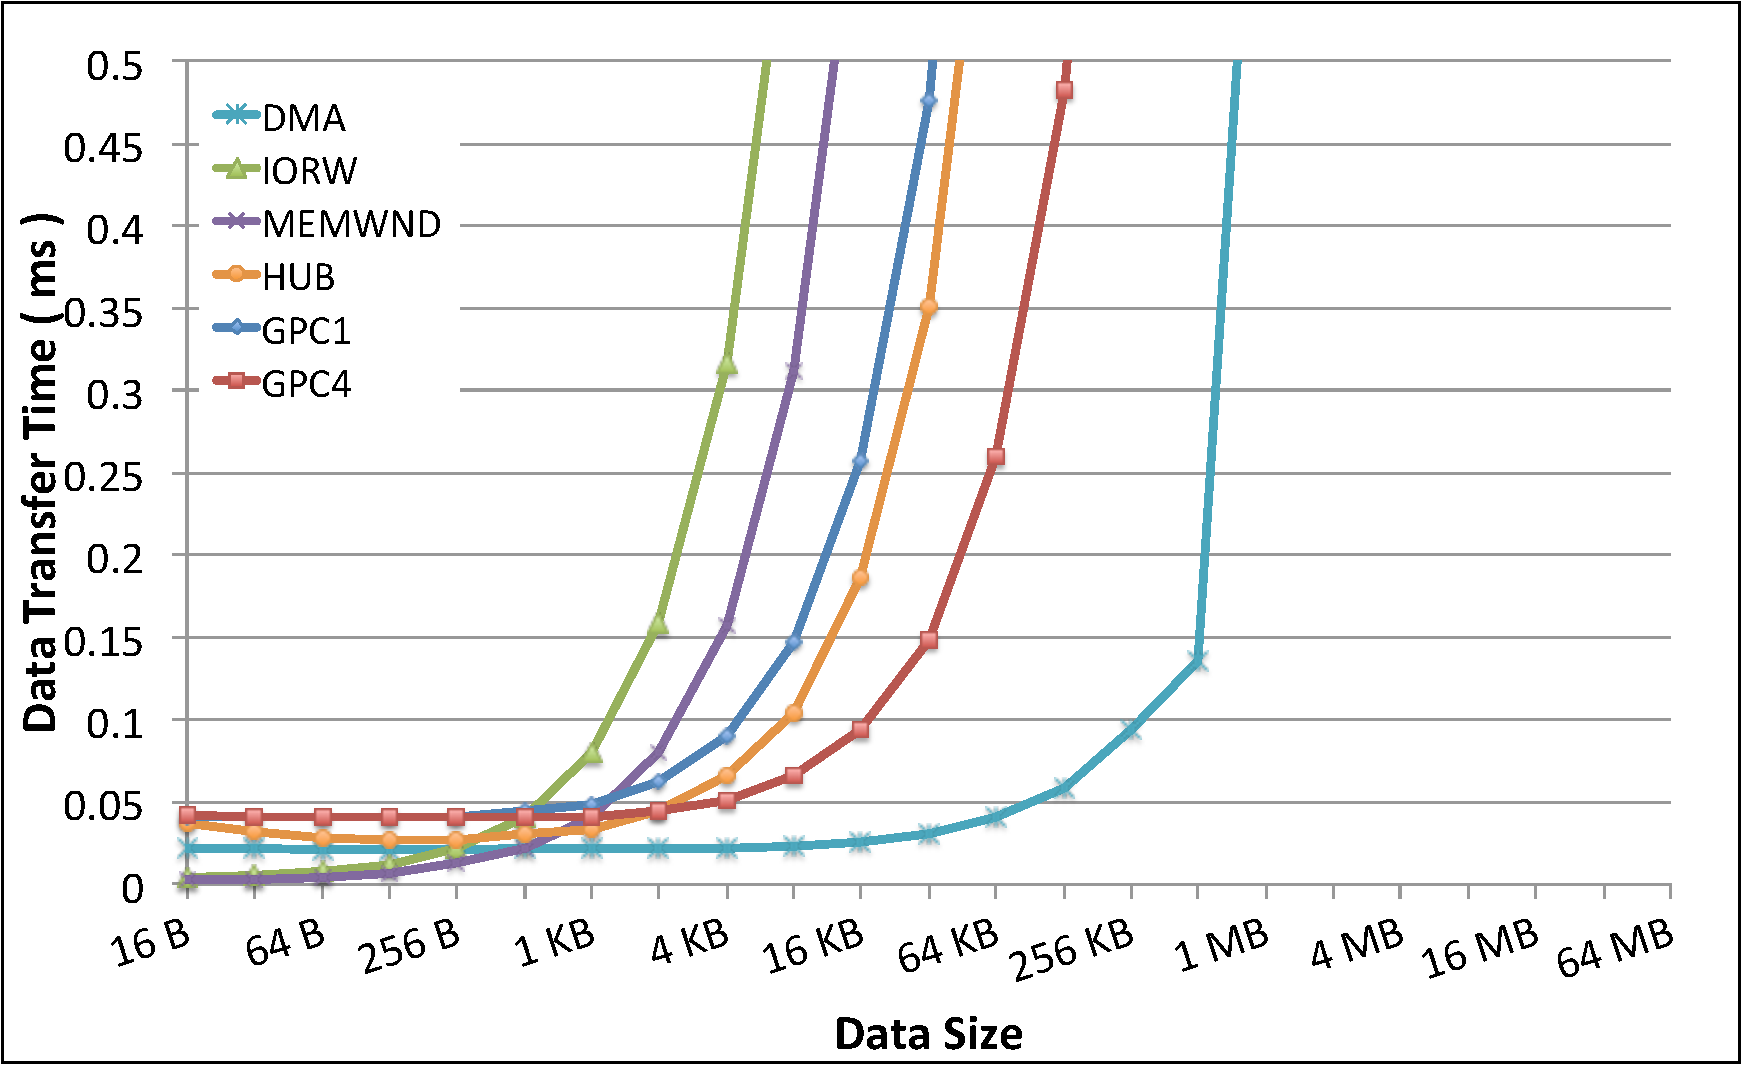
\includegraphics[width=0.34\textwidth]{figure/Graph/realtask/Memcpy_rtask_cpuload_DtoH.pdf}}
  \caption{Average performance of each data transfer method with a
  real-time task under high CPU load.}
  \label{fig:average_realtime_cpuload}
 \end{center}
 \vspace{0.5em}
 \begin{center}
  \subfigure[Host to Device]{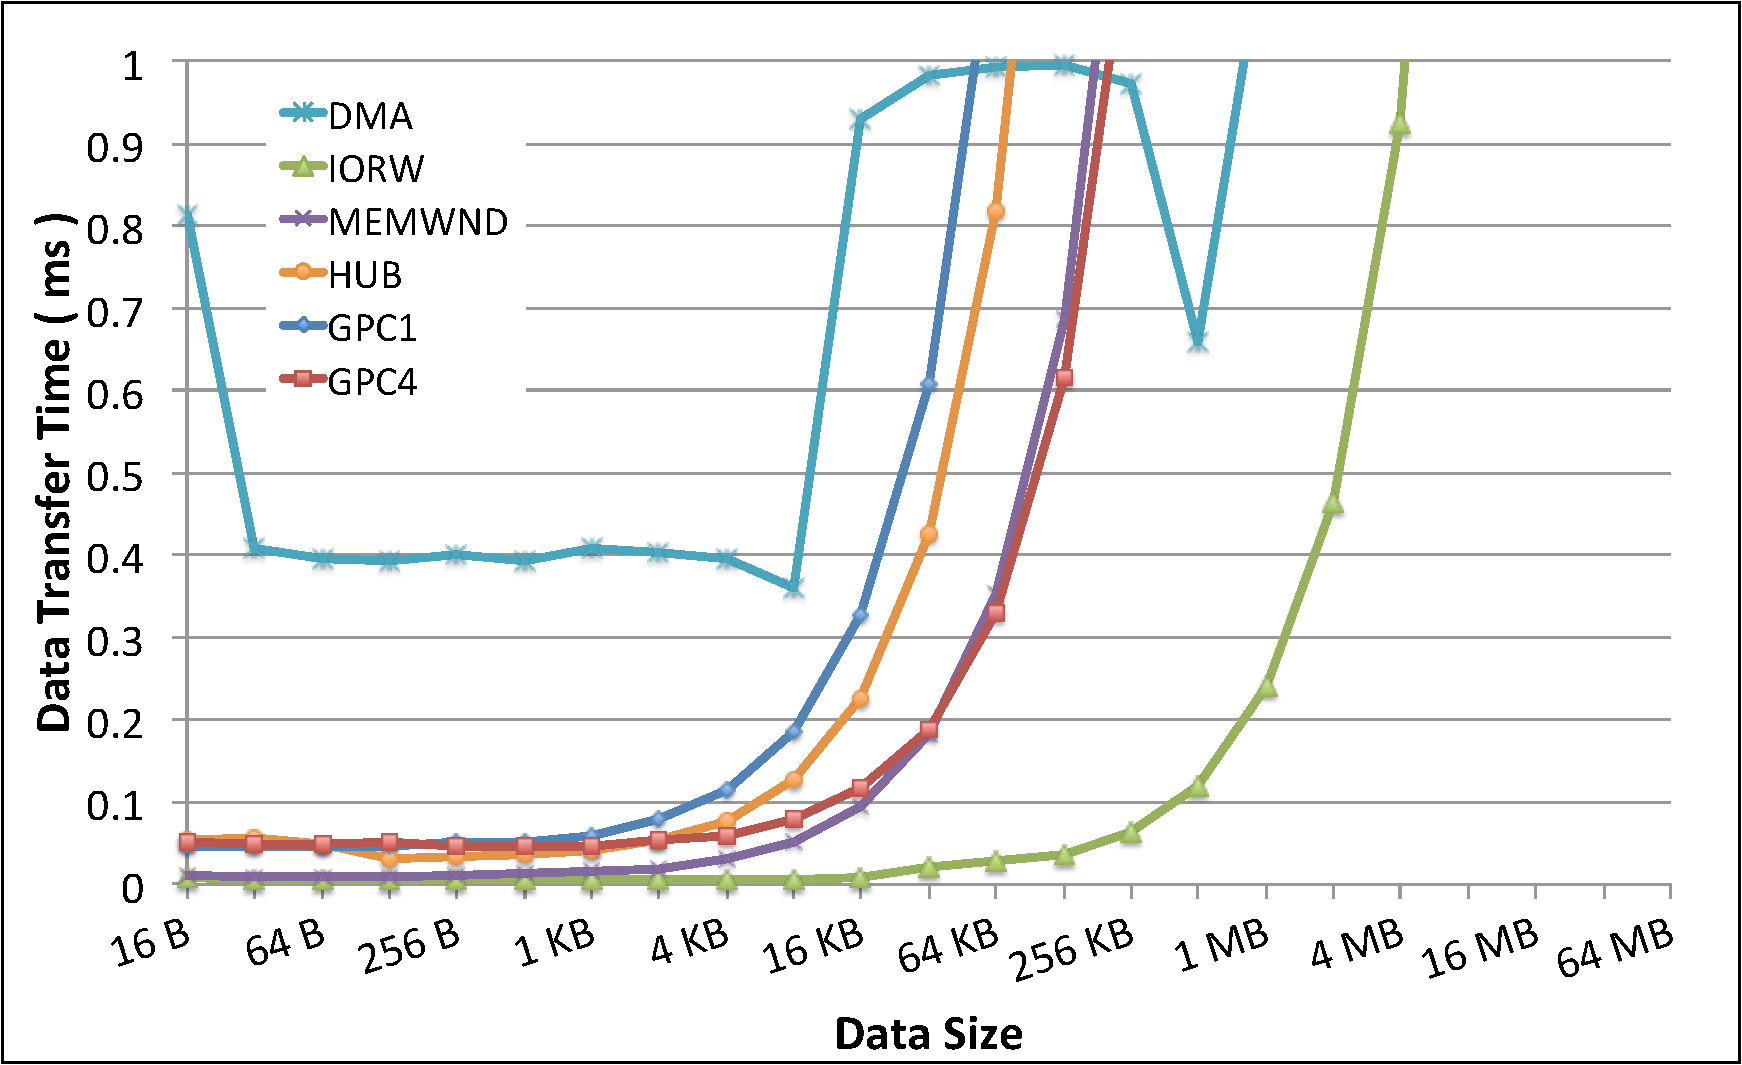
\includegraphics[width=0.34\textwidth]{figure/Graph/realtask/Memcpy_rtask_cpuload_HtoD_worst.pdf}}\\
  \subfigure[Device to Host]{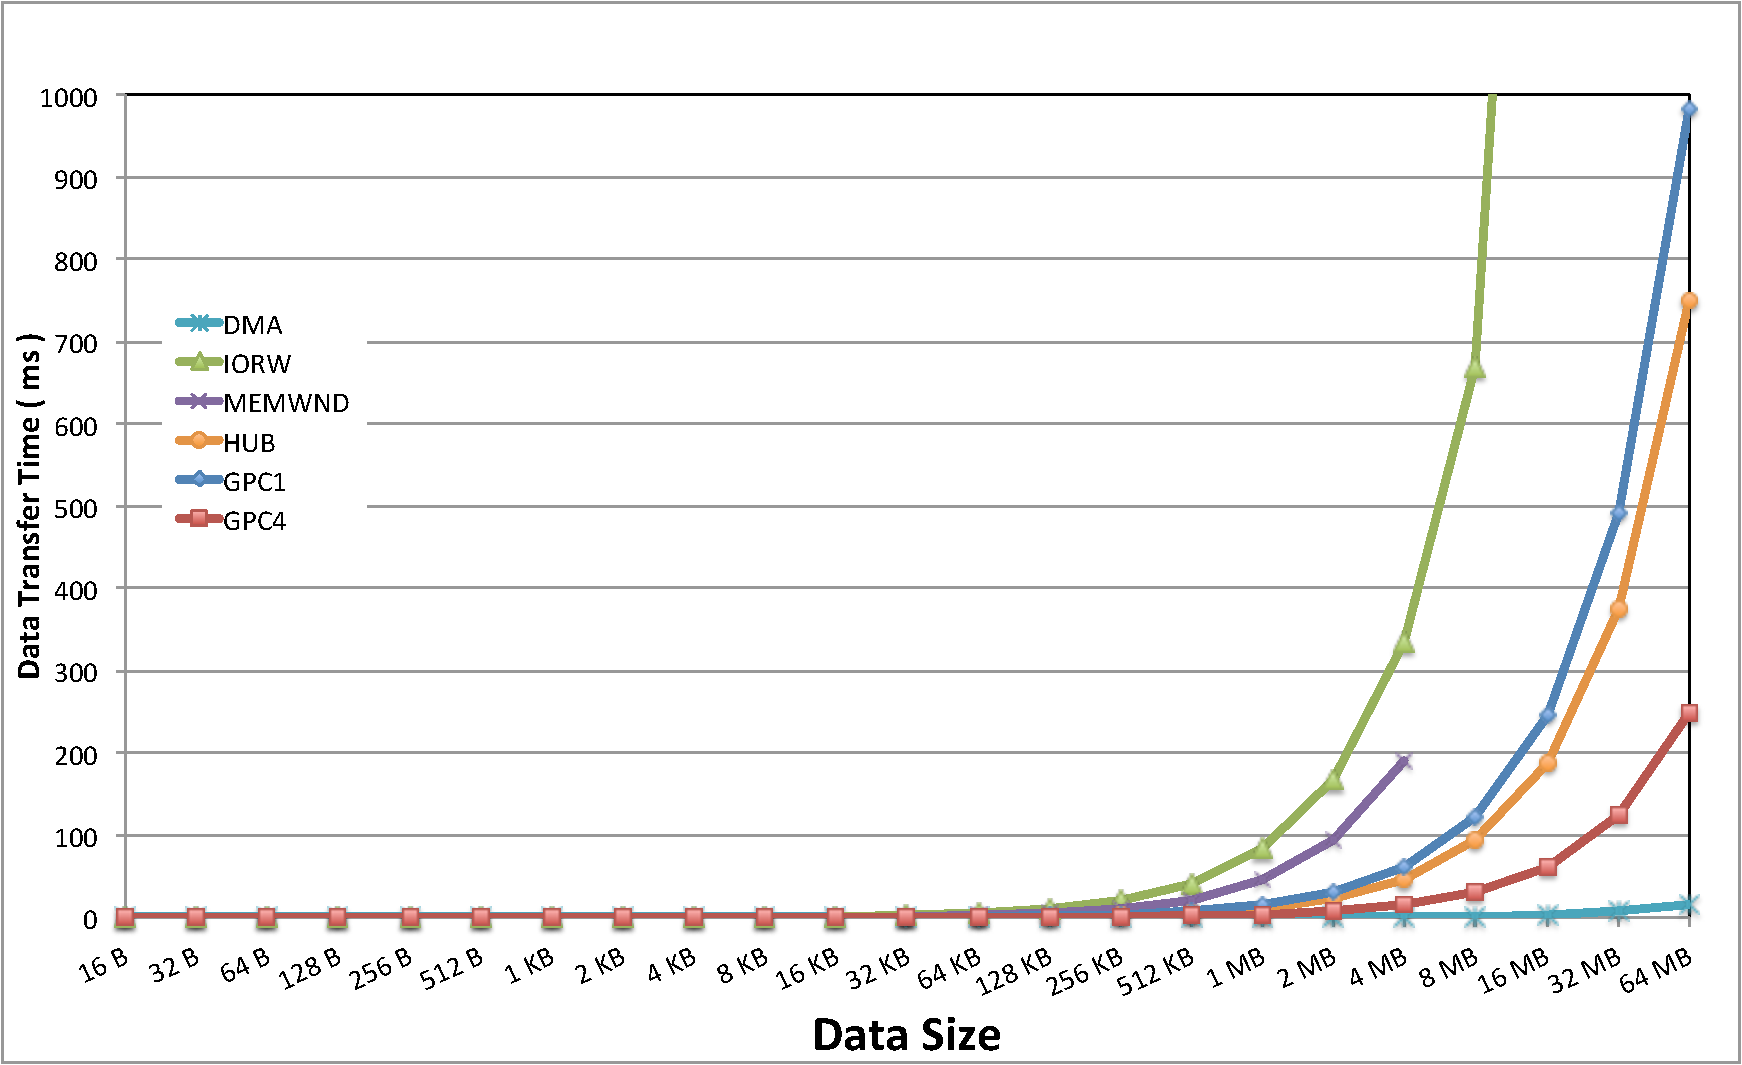
\includegraphics[width=0.34\textwidth]{figure/Graph/realtask/Memcpy_rtask_cpuload_DtoH_worst.pdf}}
  \caption{Worst-case performance of each data transfer methods with a
  real-time task under high CPU load.}
  \label{fig:worst_realtime_cpuload}
  \end{center}
\end{figure}

Figure~\ref{fig:average_realtime_cpuload} shows the average performance
of each data transfer method when a real-time task encounters extremely
high workload on the CPU.
All the methods are successfully protected from performance interference
due to the real-time scheduler.
Note that \textsf{DMA} shows a better performance than the previous
experiments despite the presence of competing workload.
This is due to the Linux real-time scheduler feature.
\textsf{DMA} is performed by GPU commands, which may impose a
suspension on the caller task.
In the Linux kernel, a real-time task is awakened in a more responsive
manner when switched from a normal task than from an idle task.
Therefore when the CPU is fully loaded by normal tasks, a real-time task
is more responsive.
The same is true for the worst-case performance as shown in
Figure~\ref{fig:worst_realtime_cpuload}.
We learn from these experiments that CPU priorities can protect the
performance of data transfer for the GPU.
Note that Gdev uses a polling approach to wait for completions of data
transfers.
An interrupt approach is also worth being investigated.

\begin{figure}[!t]
 \begin{center}
  \subfigure[Host to Device]{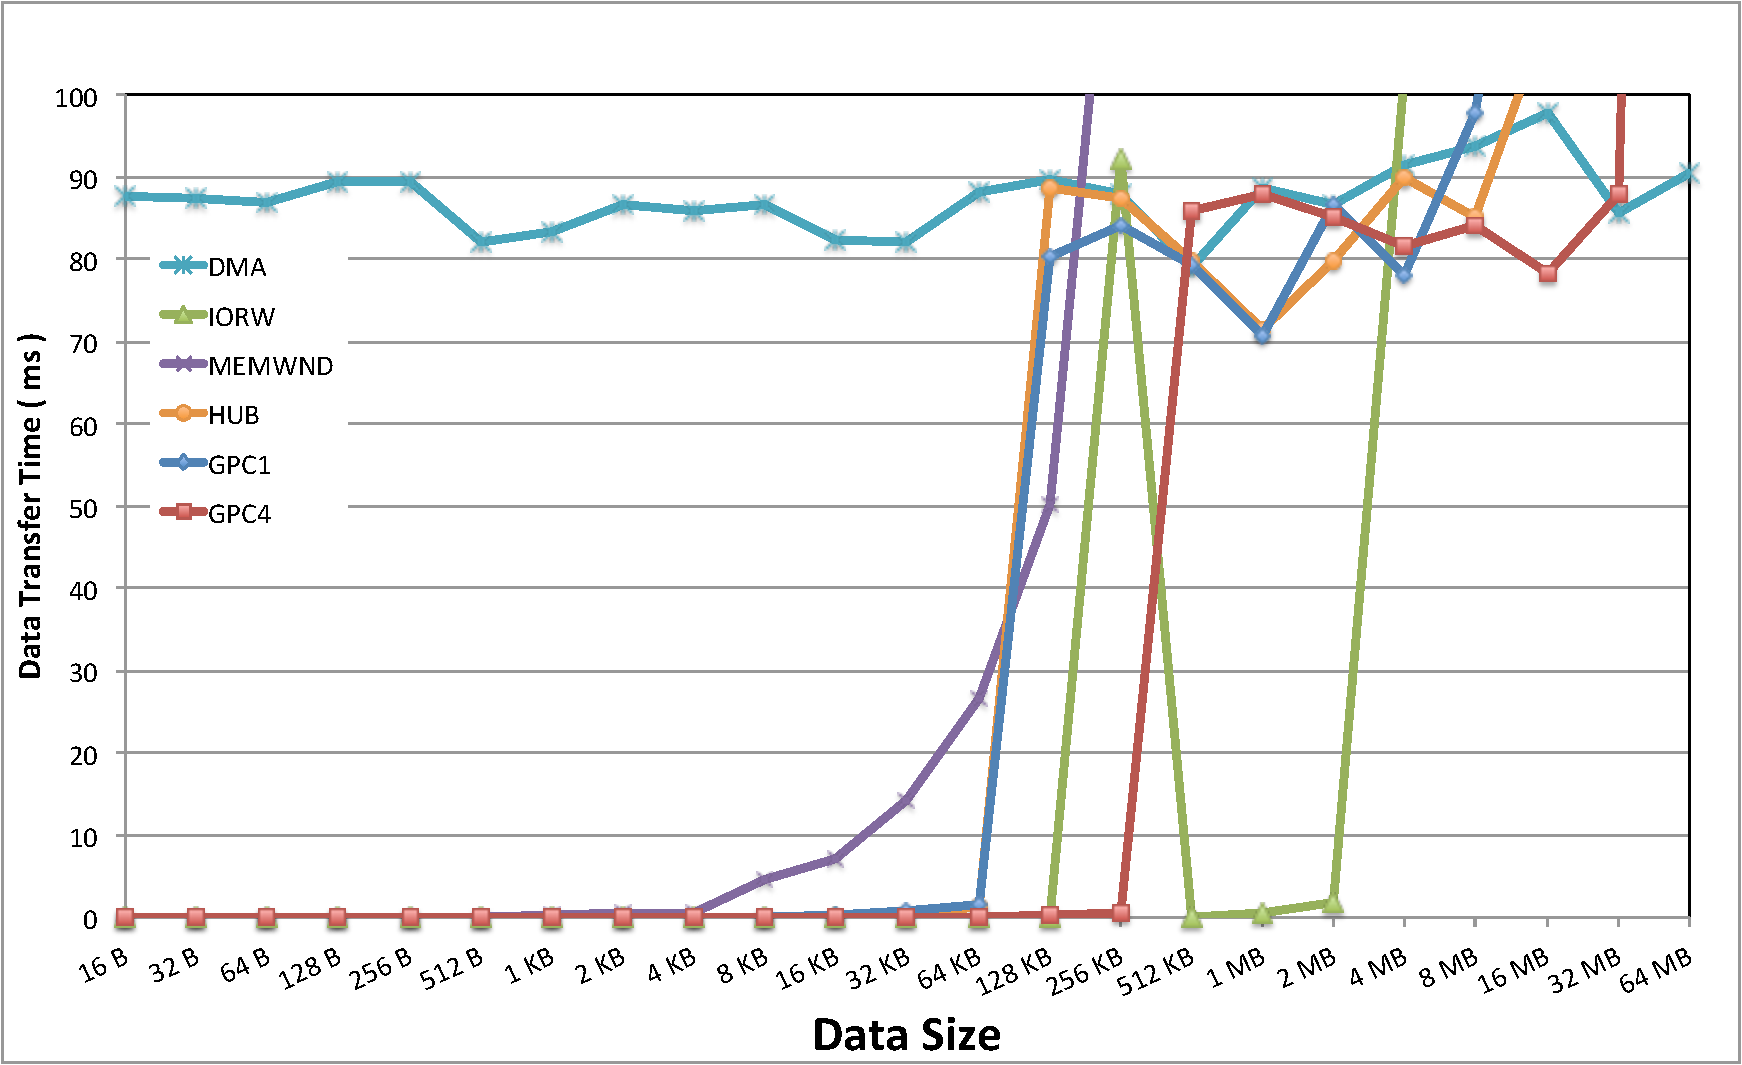
\includegraphics[width=0.34\textwidth]{figure/Graph/not_realtask/Memcpy_cpuload_HtoD.pdf}}\\
  \subfigure[Device to Host]{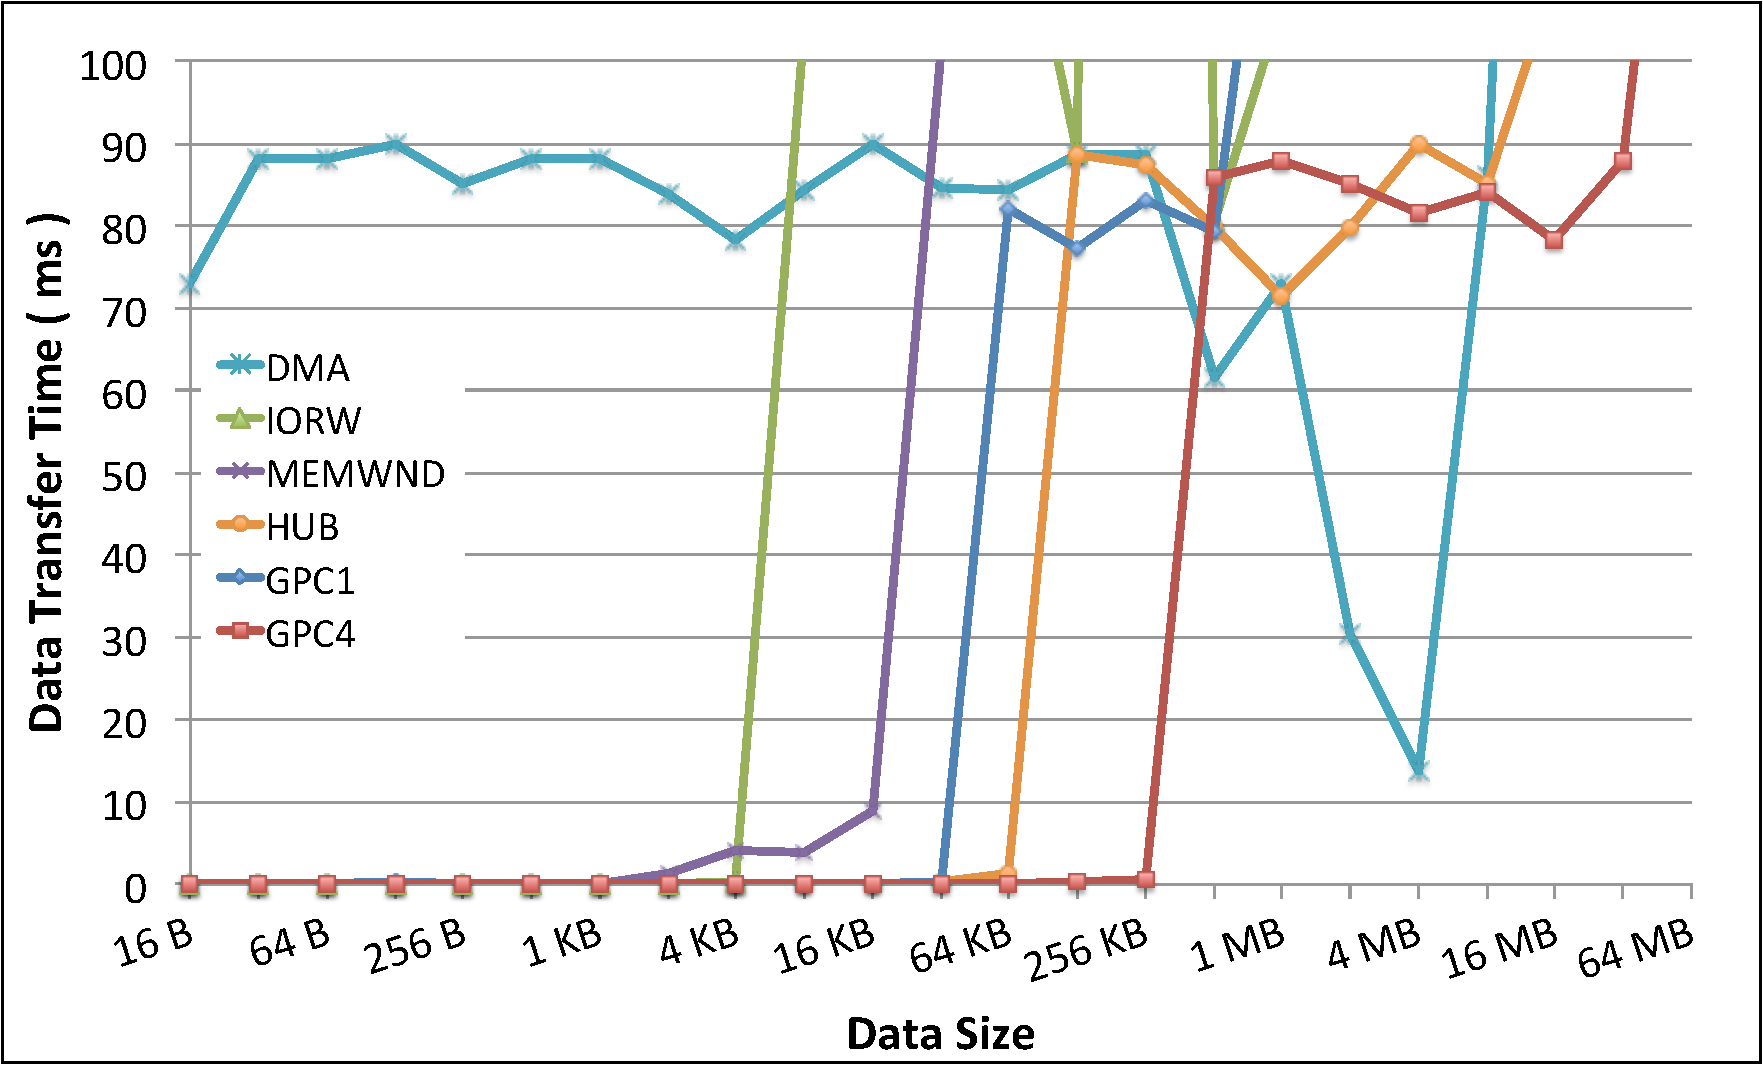
\includegraphics[width=0.34\textwidth]{figure/Graph/not_realtask/Memcpy_cpuload_DtoH.pdf}}
  \caption{Average performance of each data transfer method with a
  normal data stream under high CPU load.}
  \label{fig:average_normal_cpuload}
 \end{center}
 \vspace{0.5em}
 \begin{center}
  \subfigure[Host to Device]{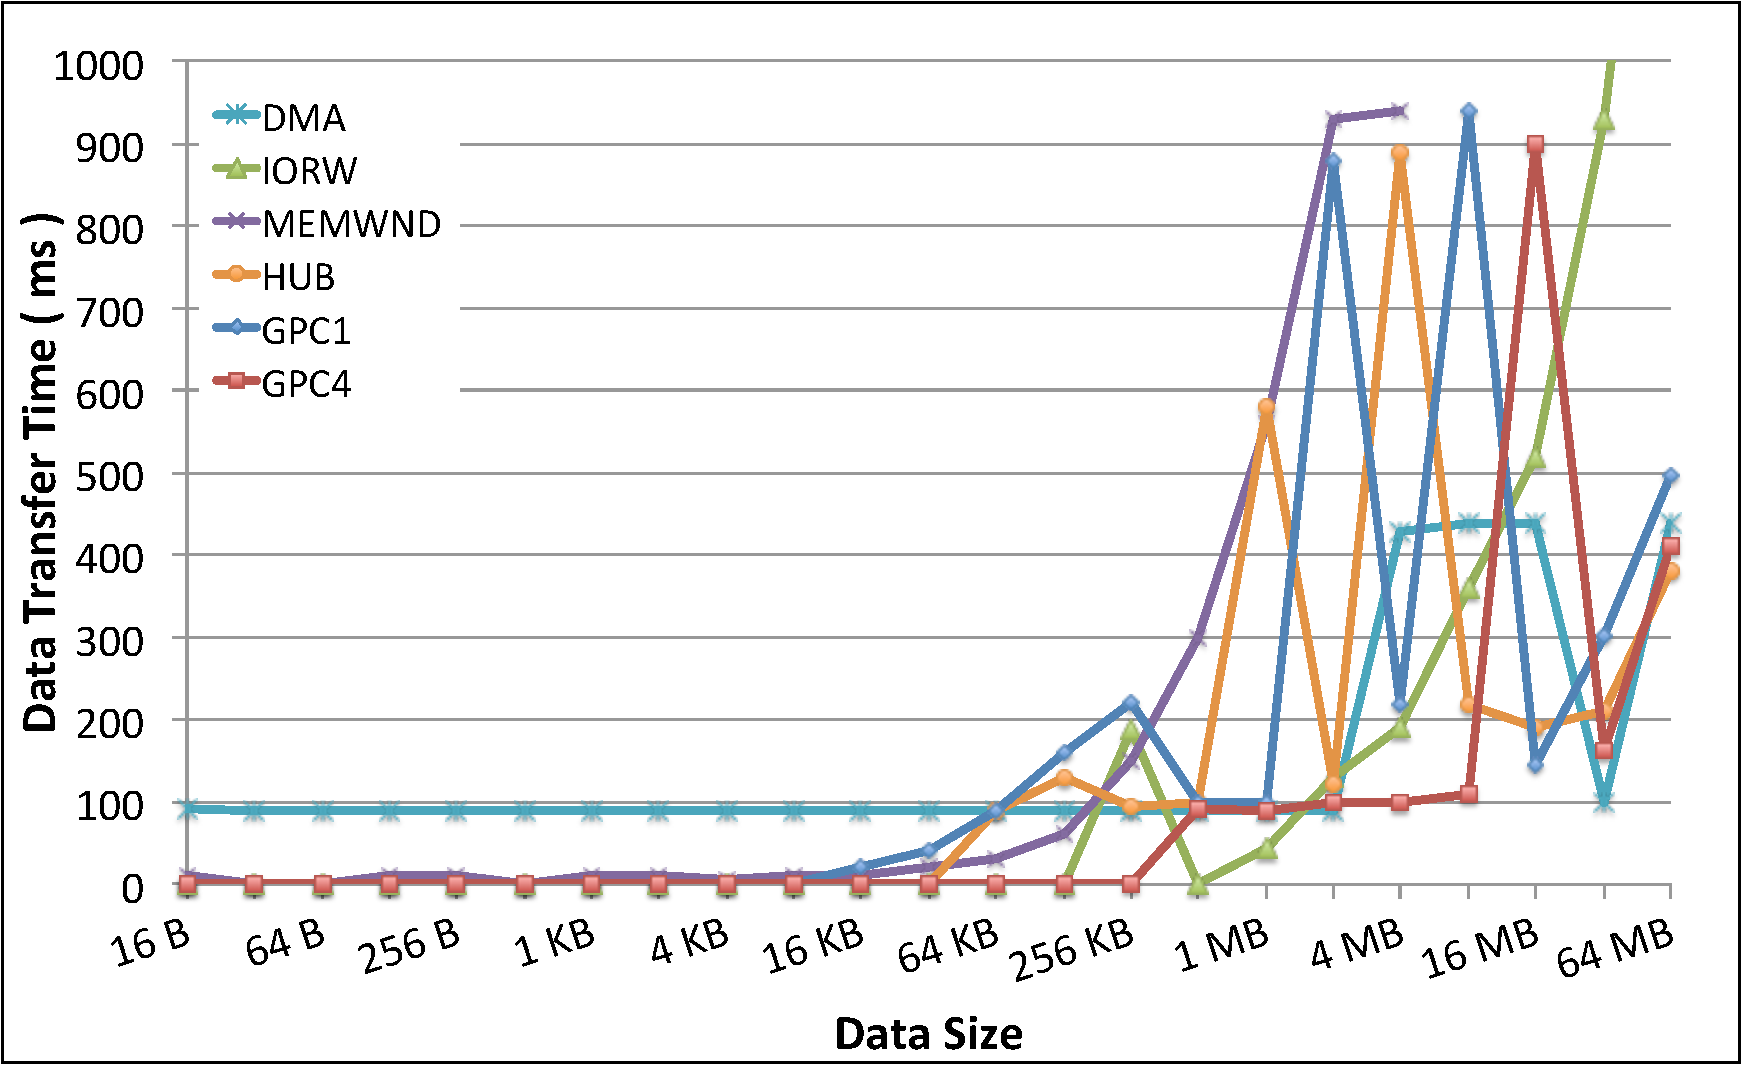
\includegraphics[width=0.34\textwidth]{figure/Graph/not_realtask/Memcpy_cpuload_HtoD_worst.pdf}}\\
  \subfigure[Device to Host]{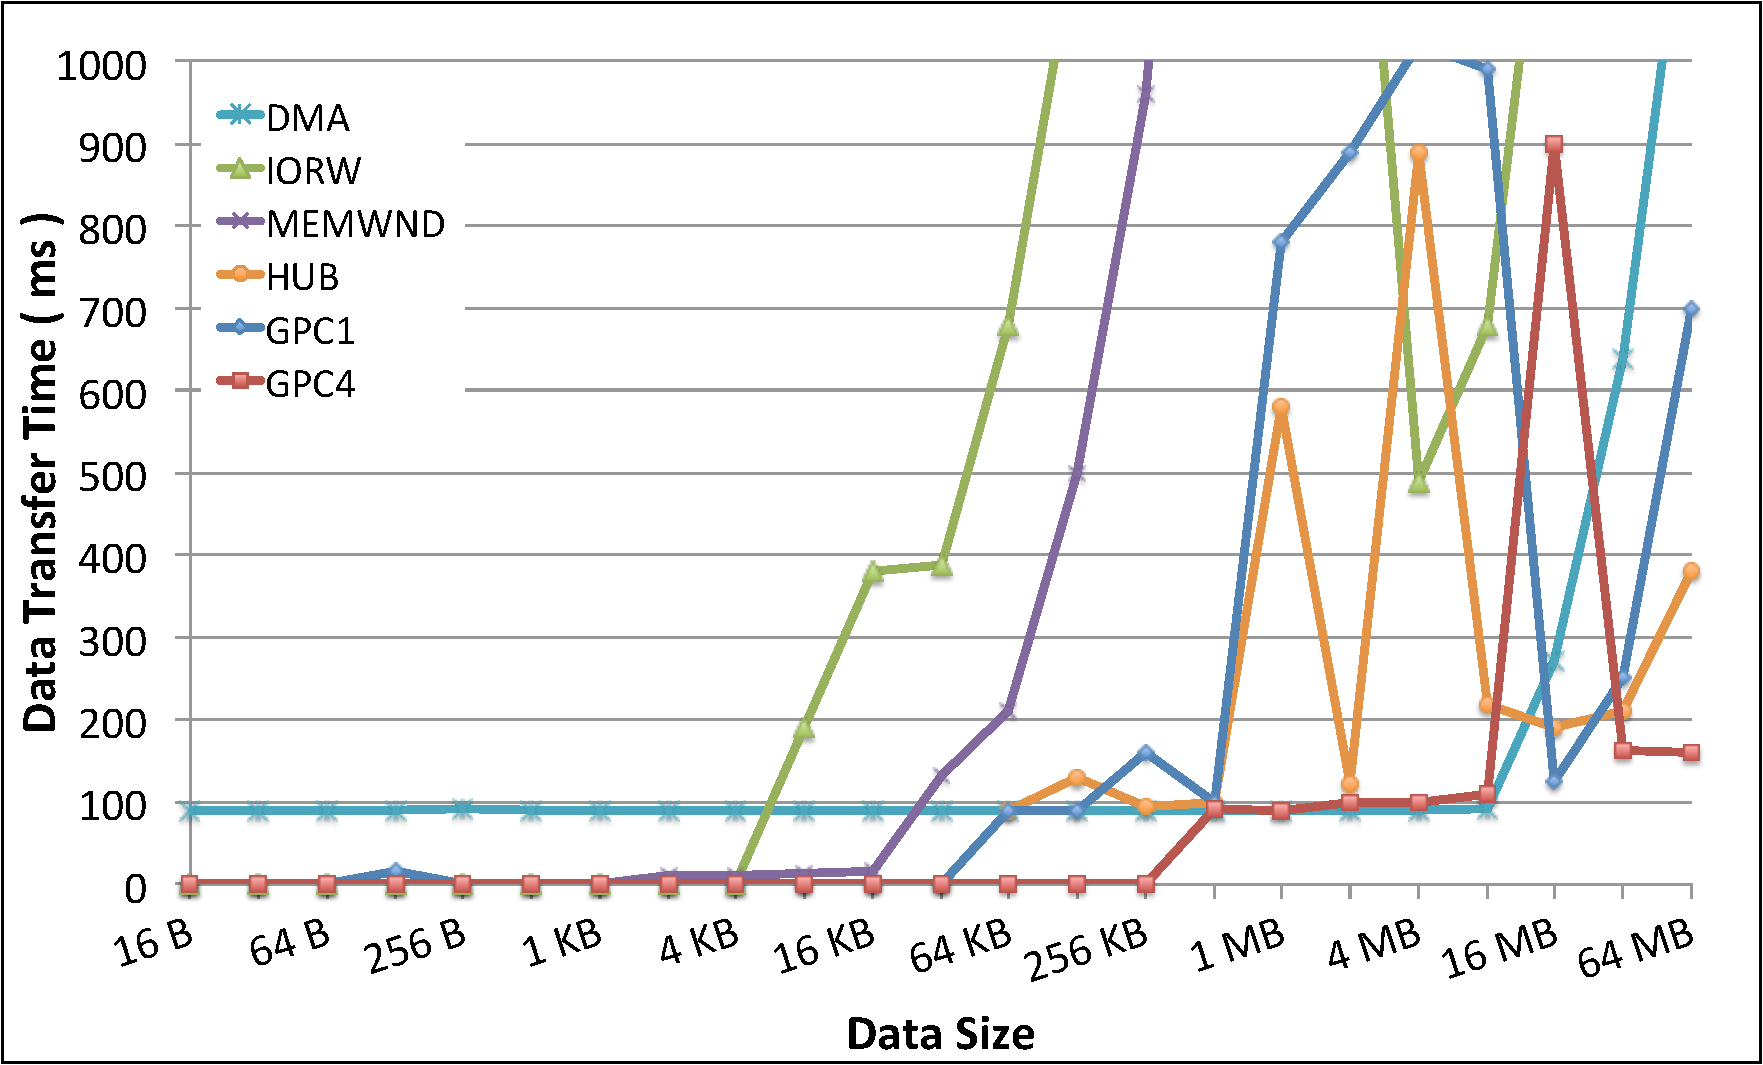
\includegraphics[width=0.34\textwidth]{figure/Graph/not_realtask/Memcpy_cpuload_DtoH_worst.pdf}}
  \caption{Worst-case performance of each data transfer method with a
  normal data stream under high CPU load.}
  \label{fig:worst_normal_cpuload}
 \end{center}
\end{figure}

For reference,
Figure~\ref{fig:average_normal_cpuload}~and~\ref{fig:worst_normal_cpuload}
show the average and the worst-case performance achieved by a normal
task when the CPU encounters extremely high workload same as the
preceding experiments.
Apparently the data transfer times increase by orders of magnitude as
compared to those achieved by a real-time task.
\textsf{DMA} shows a bad performance for small data while it can sustain
that performance for large data.
This is attributed to the fact that once a DMA command is fired, the
data transfer does not have to compete with CPU workload.
The other methods are more or less controlled by the CPU, and thus are
more affected by CPU workload.
This finding provides a design choice for the system implementation.

\begin{figure}[!t]
 \begin{center}
  \subfigure[Host to Device]{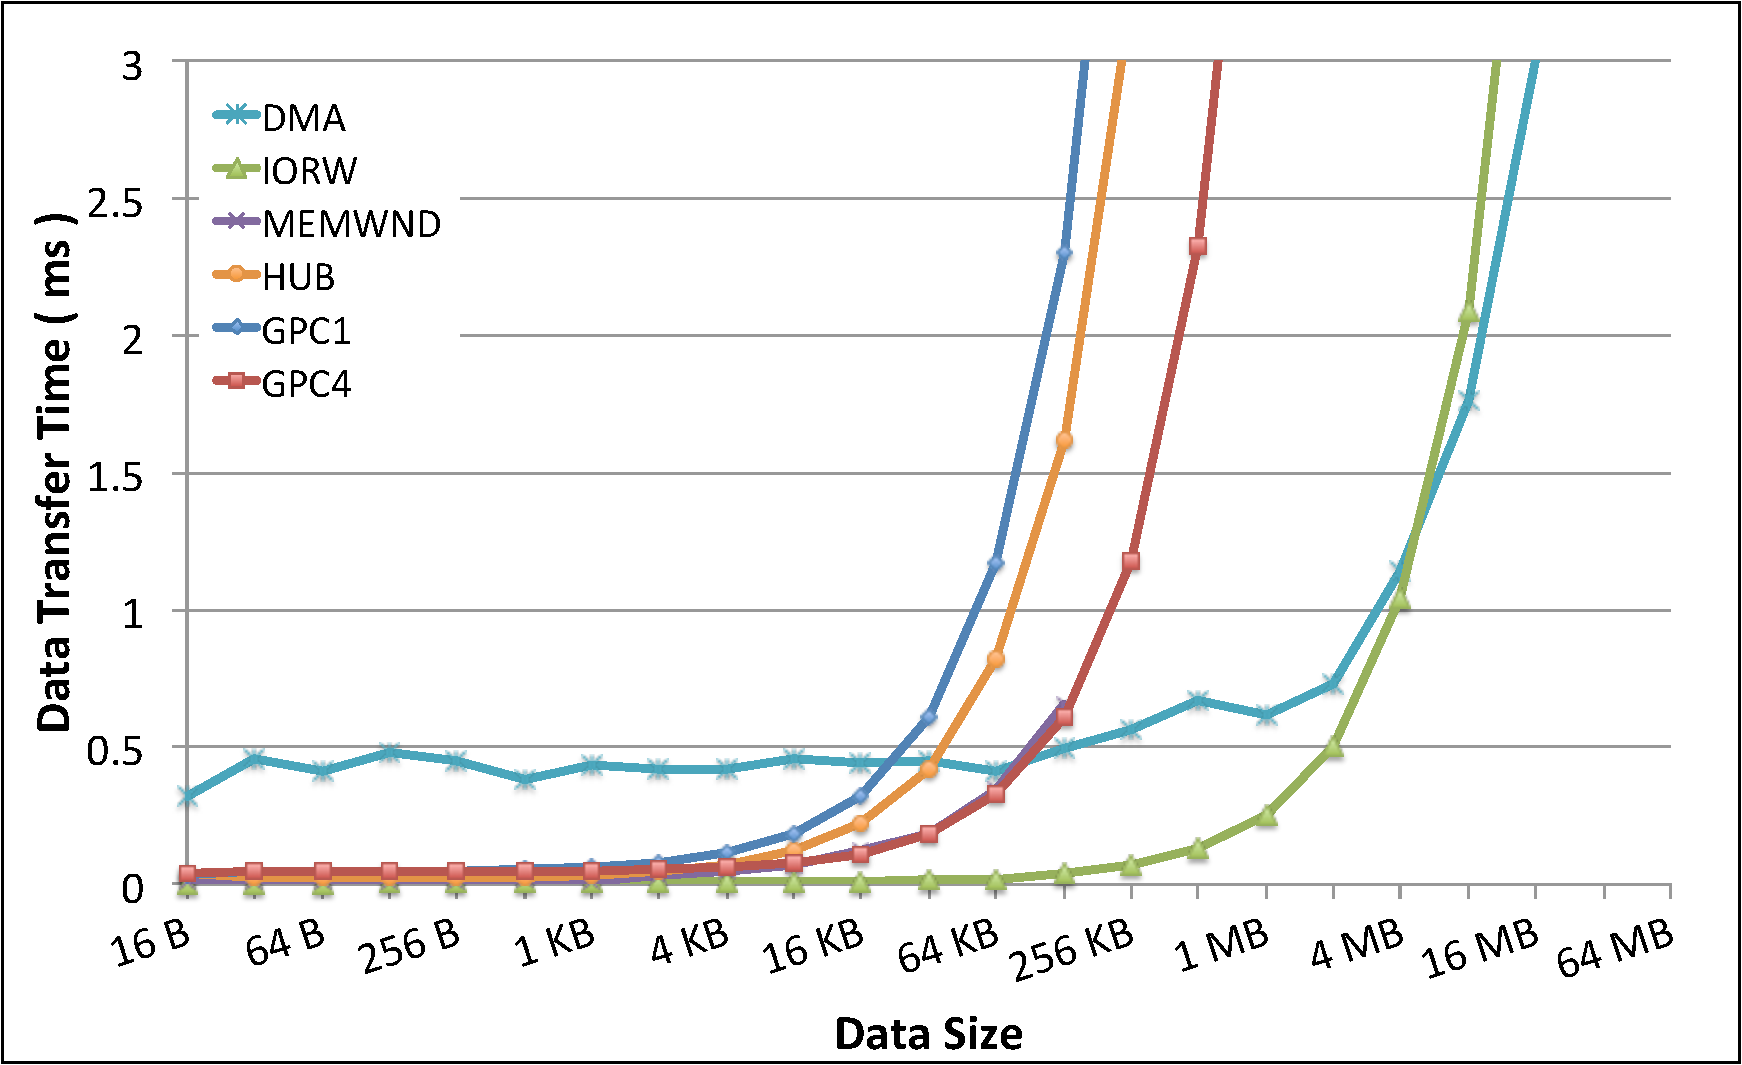
\includegraphics[width=0.34\textwidth]{figure/Graph/realtask/Memcpy_rtask_memswap_HtoD.pdf}}\\
  \subfigure[Device to Host]{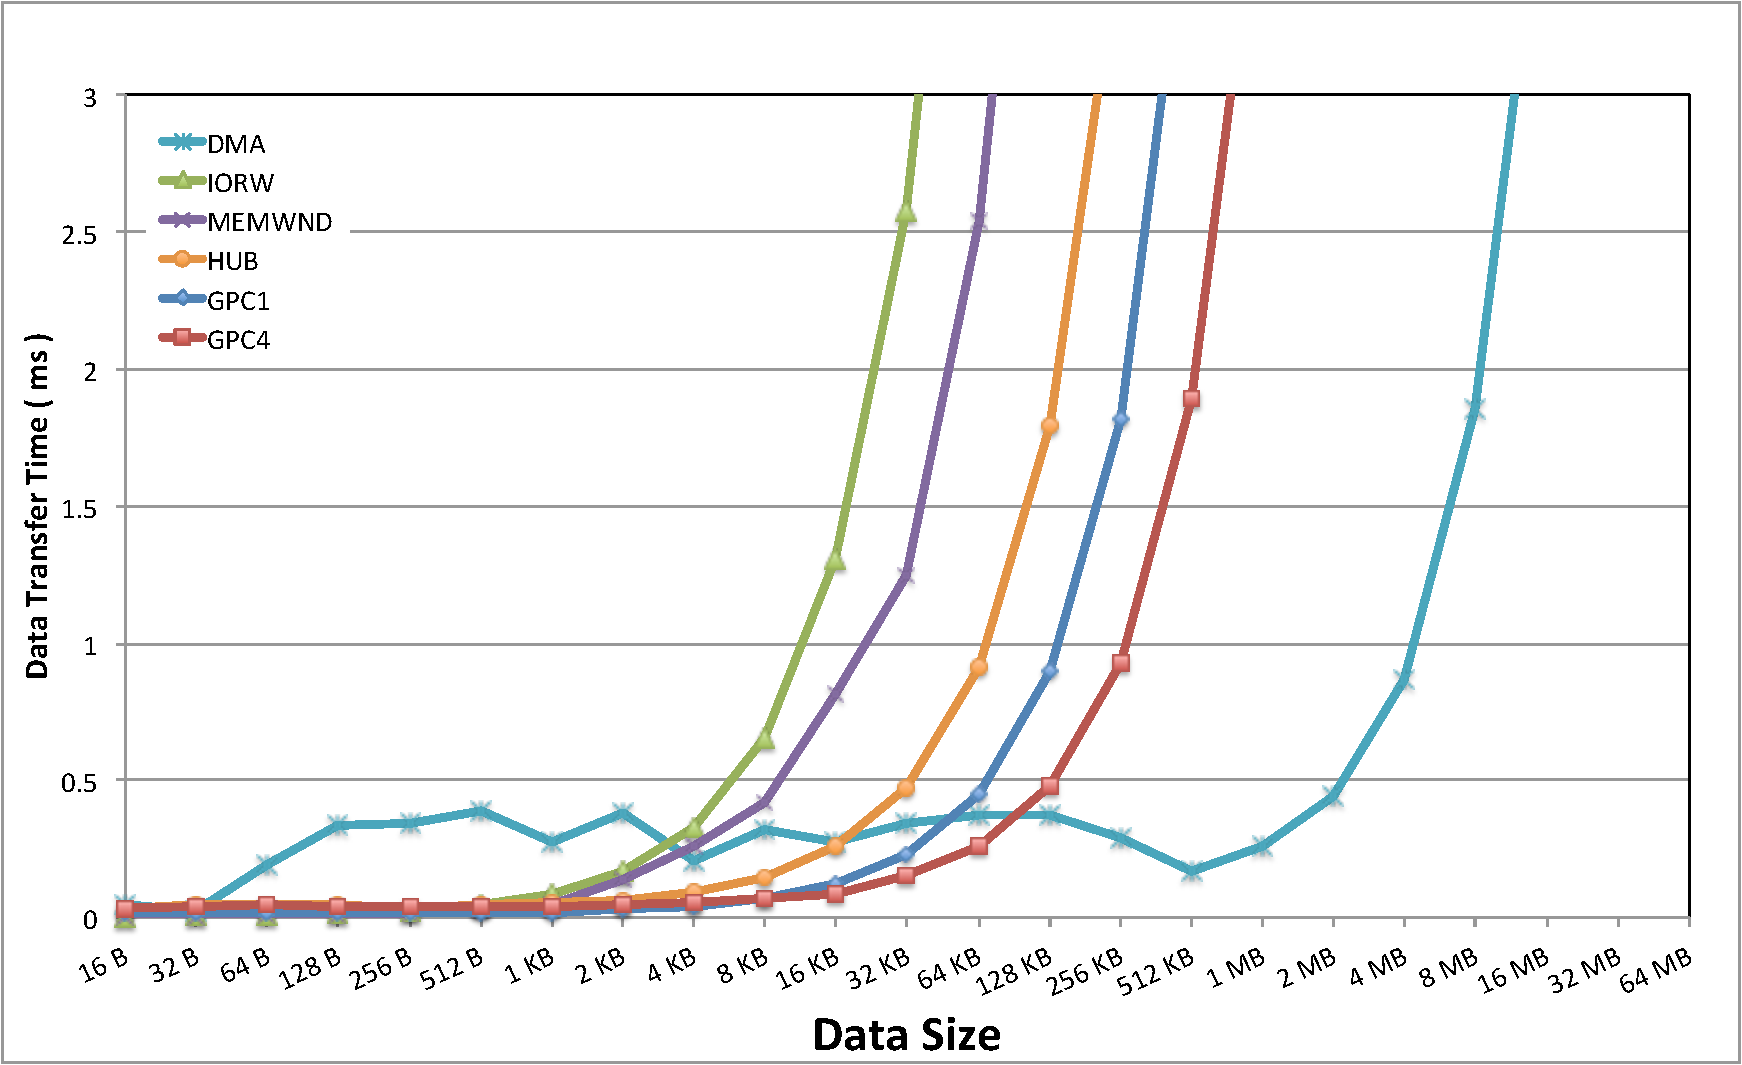
\includegraphics[width=0.34\textwidth]{figure/Graph/realtask/Memcpy_rtask_memswap_DtoH.pdf}}
  \caption{Average performance of each data transfer method with a
  real-time task under high memory pressure.}
  \label{fig:average_realtime_memswap}
 \end{center}
 \vspace{0.5em}
 \begin{center}
  \subfigure[Host to Device]{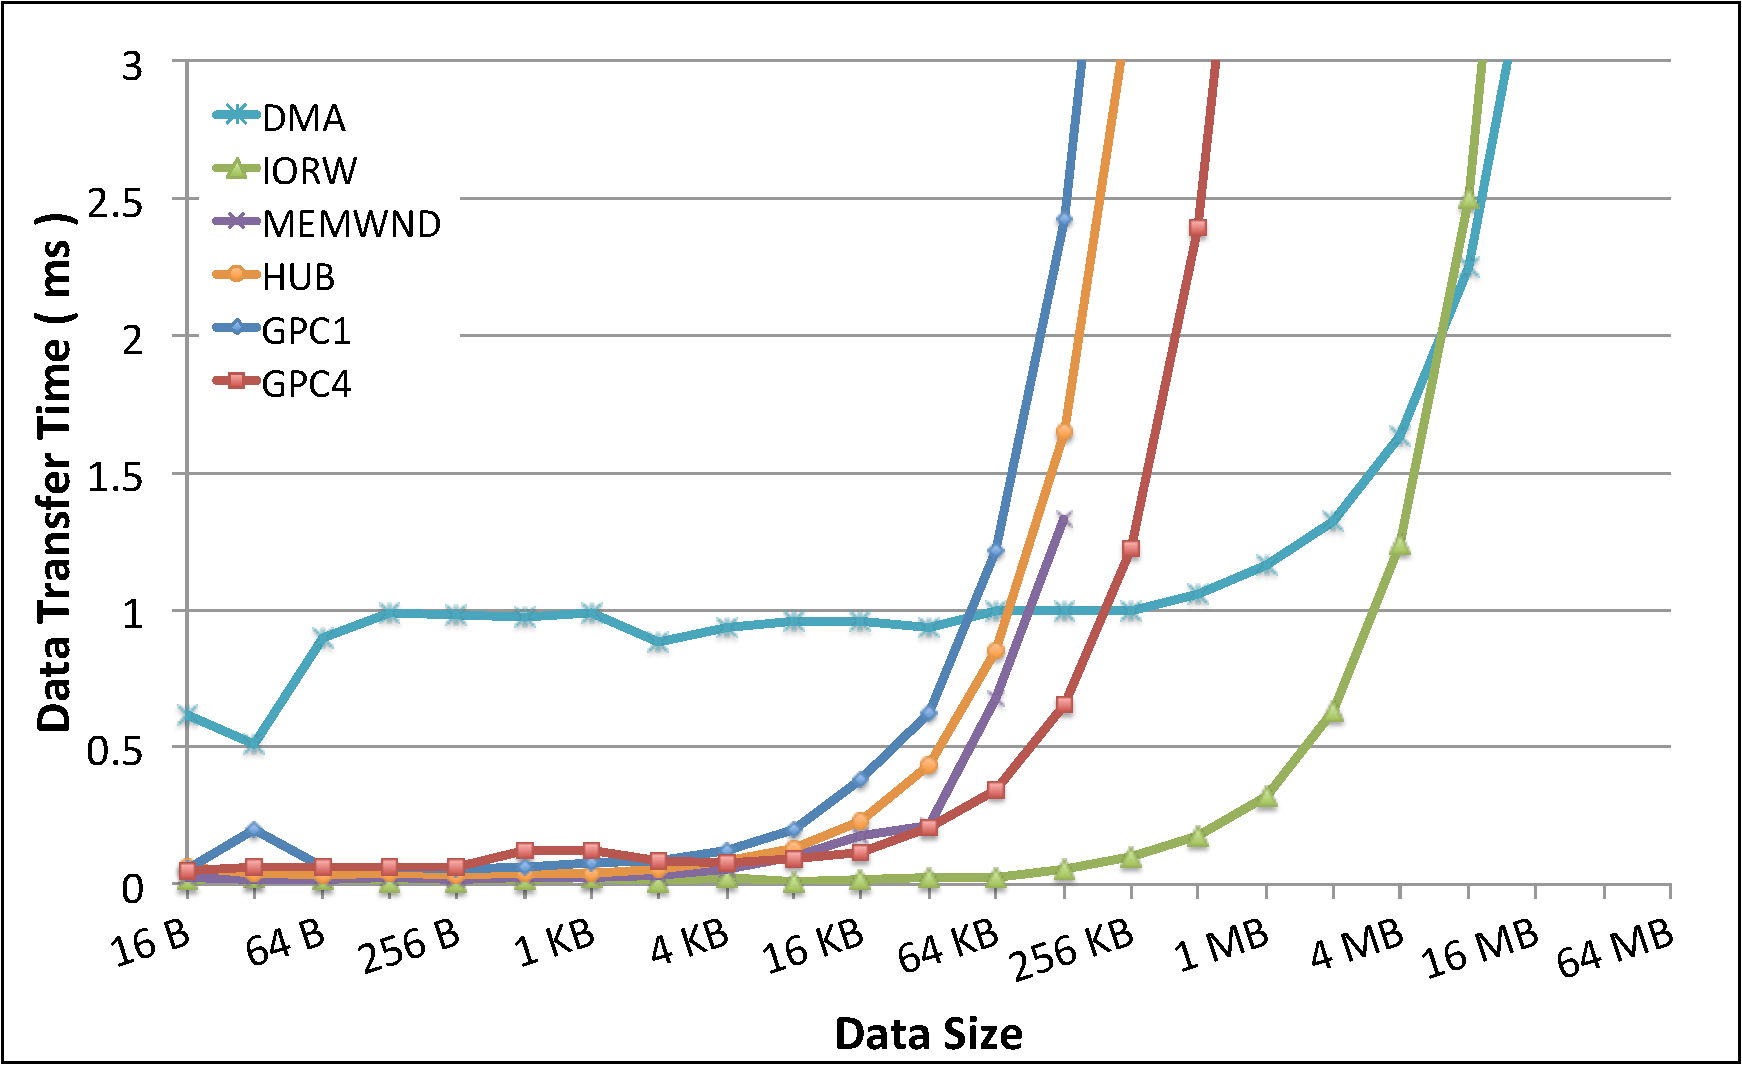
\includegraphics[width=0.34\textwidth]{figure/Graph/realtask/Memcpy_rtask_memswap_HtoD_worst.pdf}}\\
  \subfigure[Device to Host]{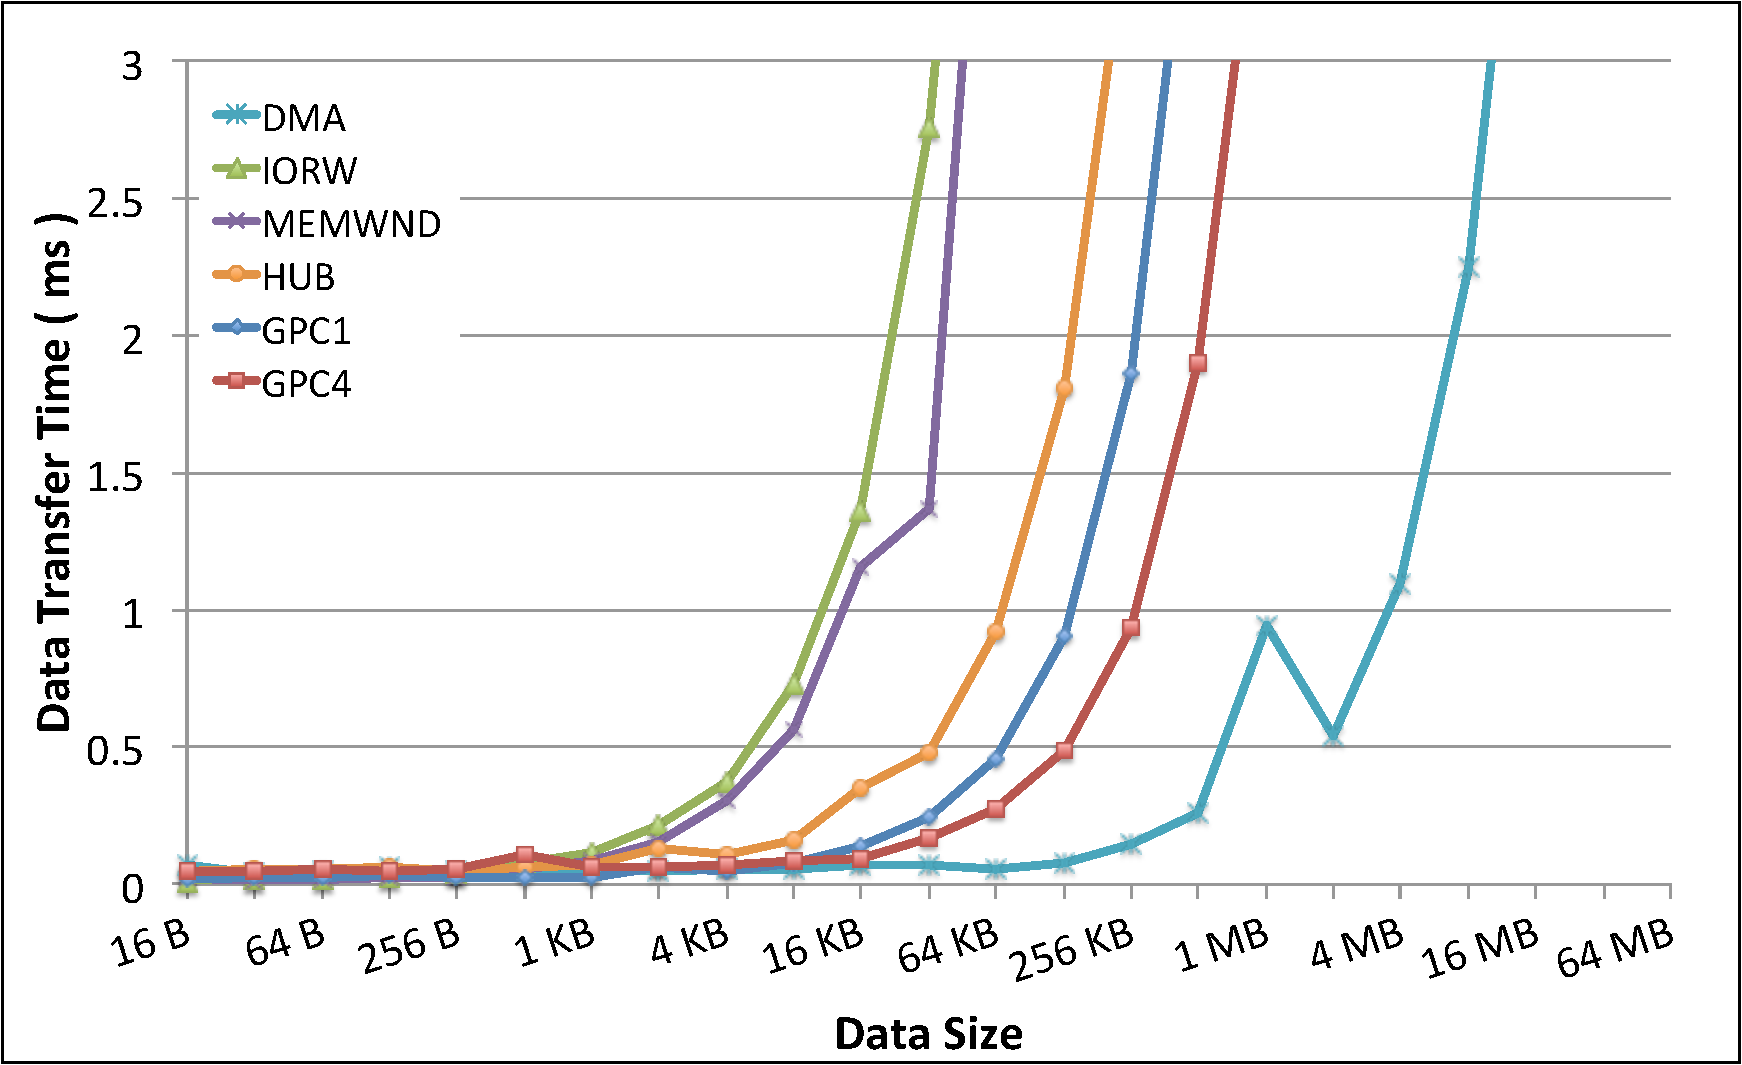
\includegraphics[width=0.34\textwidth]{figure/Graph/realtask/Memcpy_rtask_memswap_DtoH_worst.pdf}}
  \caption{Worst-case performance of each data transfer method with a
  real-time task under high memory pressure.}
  \label{fig:worst_realtime_memswap}
 \end{center}
\end{figure}

From now on, we restrict our attention to a real-time task.
We next evaluate the performance of each data transfer method under high
memory pressure, creating another task that eats up host memory space.
In some sense, this is not a meaningful experiment because we use the
pinned host memory space to allocate buffers while the memory pressure
is supposed to compel the paged host memory space.
Having said that, the memory pressure could still impose indirect
interference on real-time tasks~\cite{Kato_RTSJ11, Yang_OSDI08}.
It is worth conducting this experiment.
As demonstrated in
Figure~\ref{fig:average_realtime_memswap}~and~\ref{fig:worst_realtime_memswap},
the impact of memory pressure on the data transfer performance is
neligible.
This means that all the data transfer methods investigated in this paper
require not much paged host memory space.
Otherwise they must be interfered by memory workload.

\begin{figure}[!t]
 \begin{center}
  \subfigure[Host to Device]{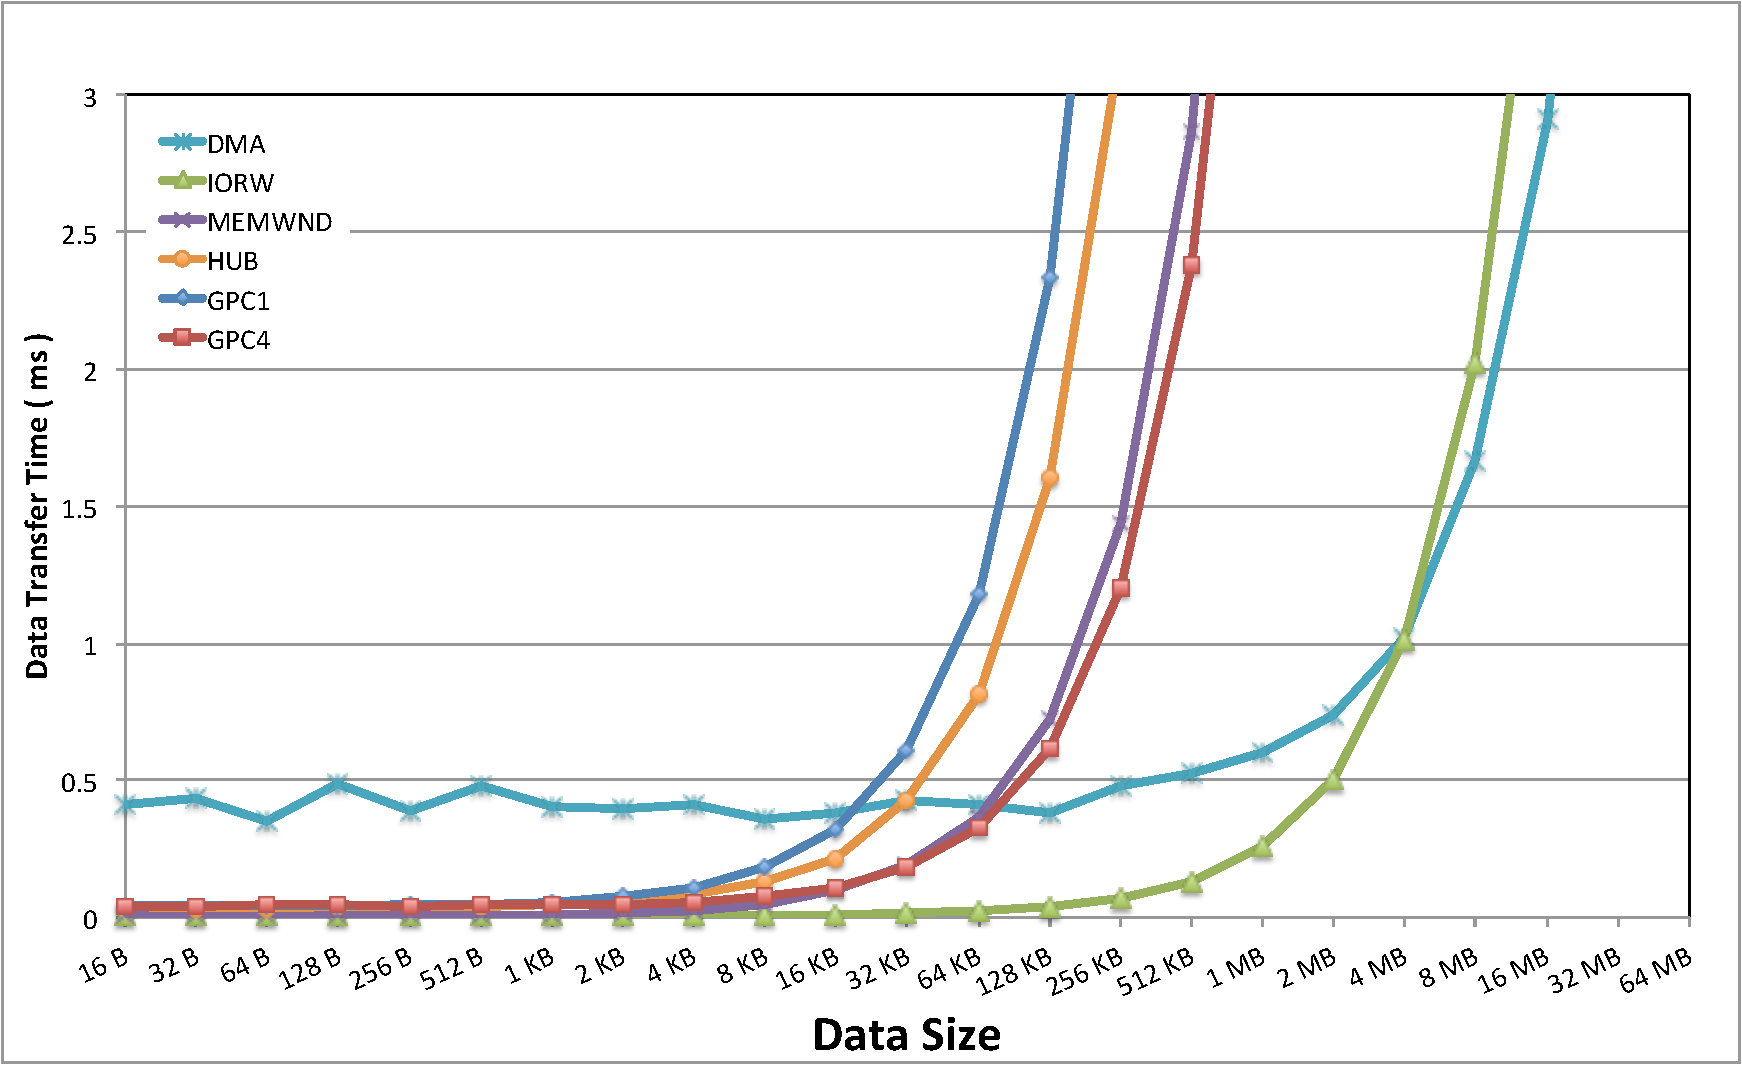
\includegraphics[width=0.34\textwidth]{figure/Graph/realtask/Memcpy_rtask_hackbench_HtoD.pdf}}\\
  \subfigure[Device to Host]{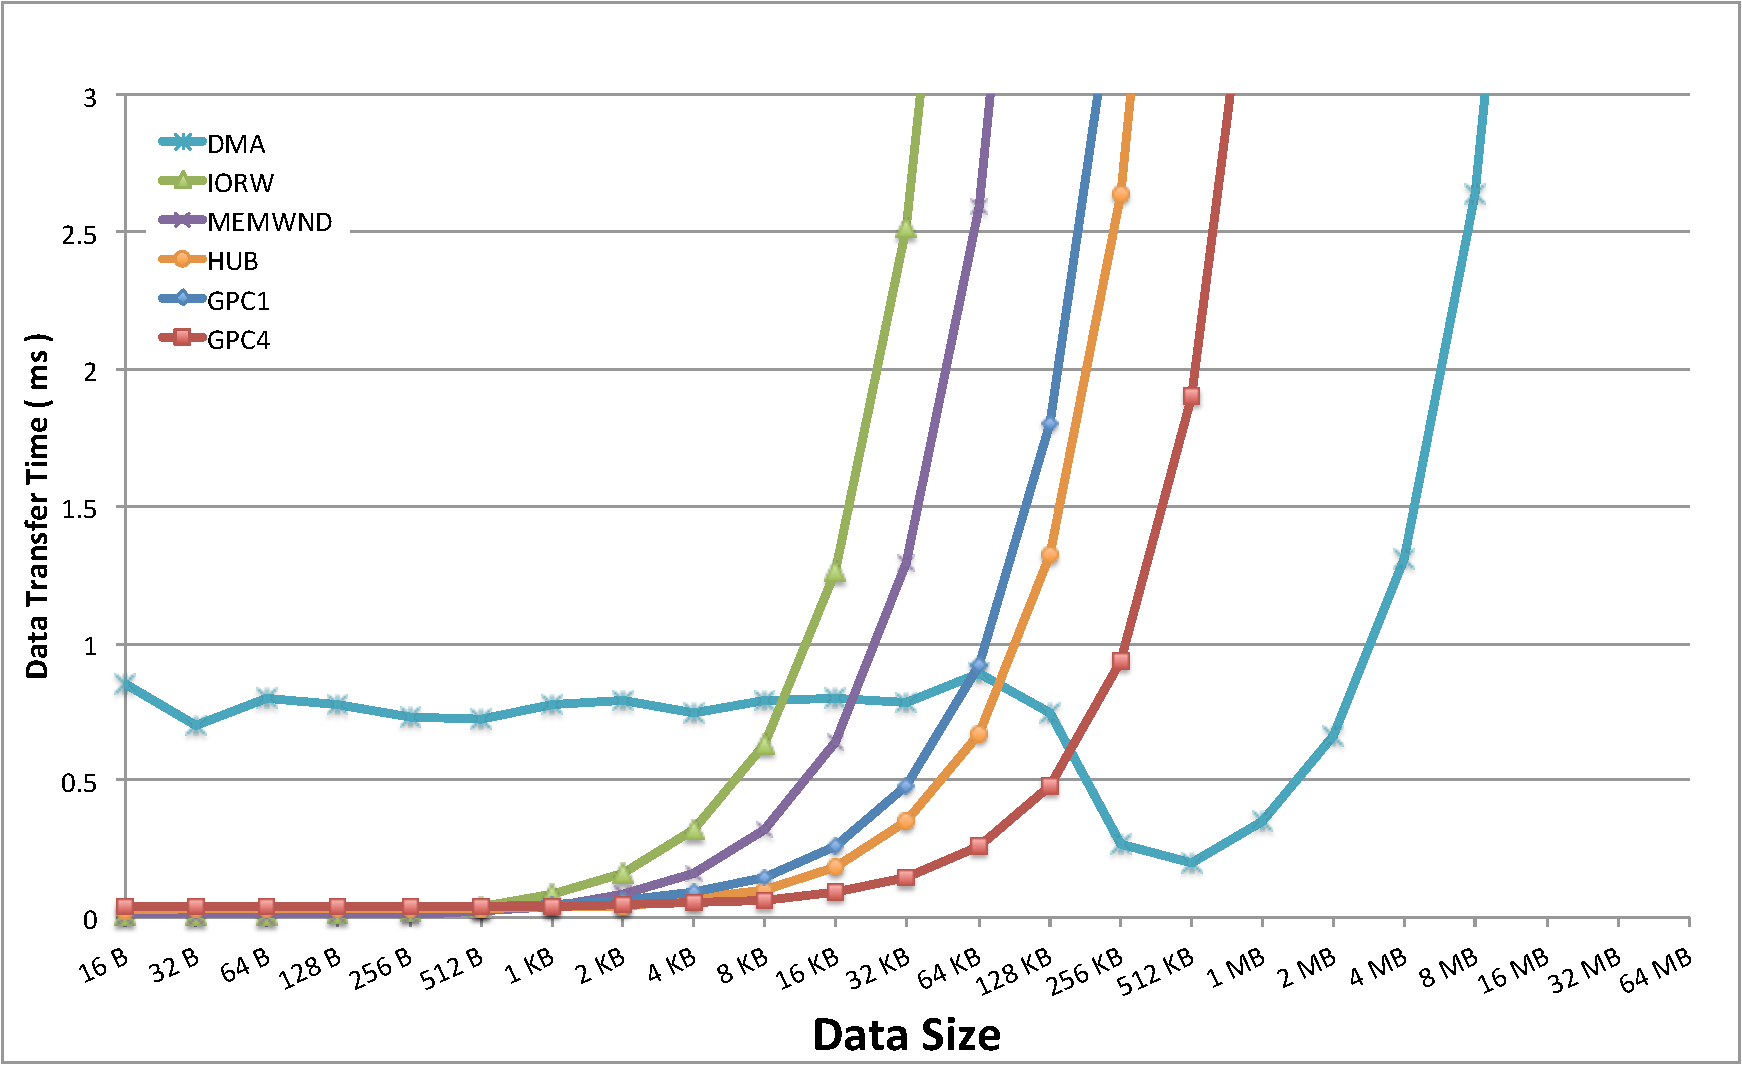
\includegraphics[width=0.34\textwidth]{figure/Graph/realtask/Memcpy_rtask_hackbench_DtoH.pdf}}
  \caption{Average performance of each data transfer method with a
  real-time task in the presence of \textsf{hackbench}.}
  \label{fig:average_realtime_hackbench}
 \end{center}
 \vspace{0.5em}
 \begin{center}
  \subfigure[Host to Device]{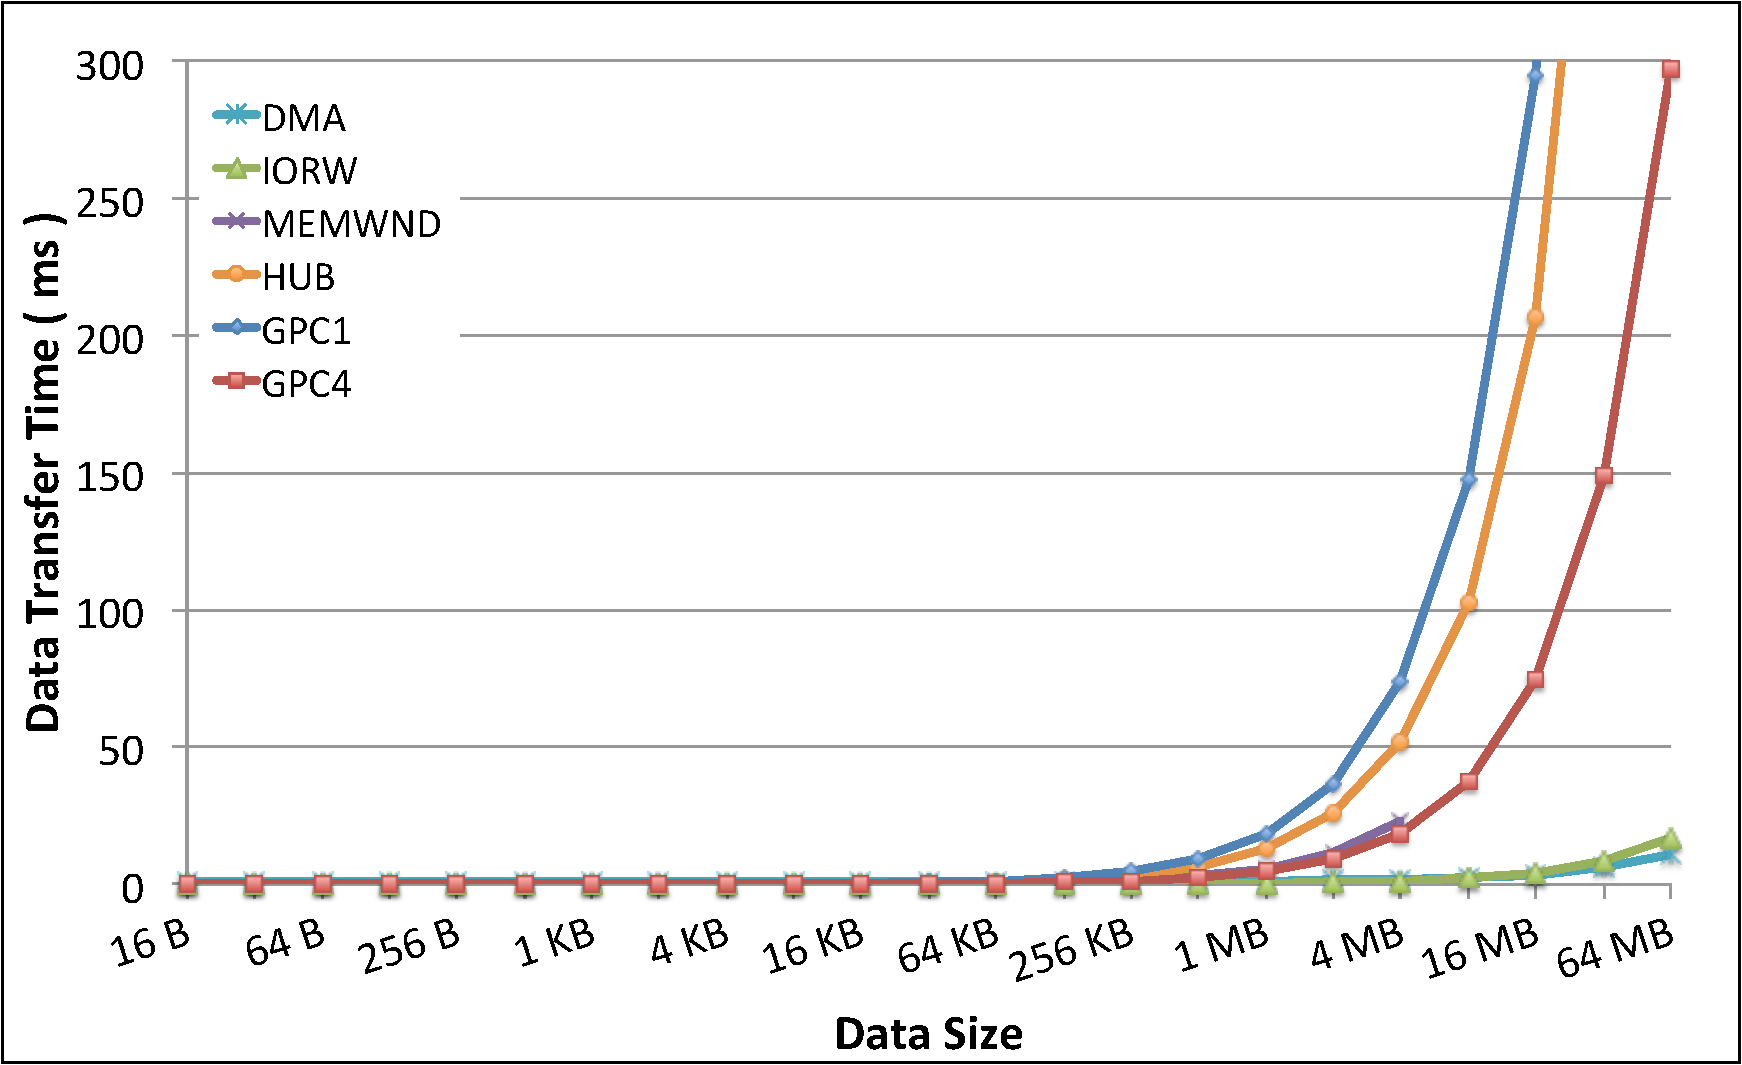
\includegraphics[width=0.34\textwidth]{figure/Graph/realtask/Memcpy_rtask_hackbench_HtoD_worst.pdf}}\\
  \subfigure[Device to Host]{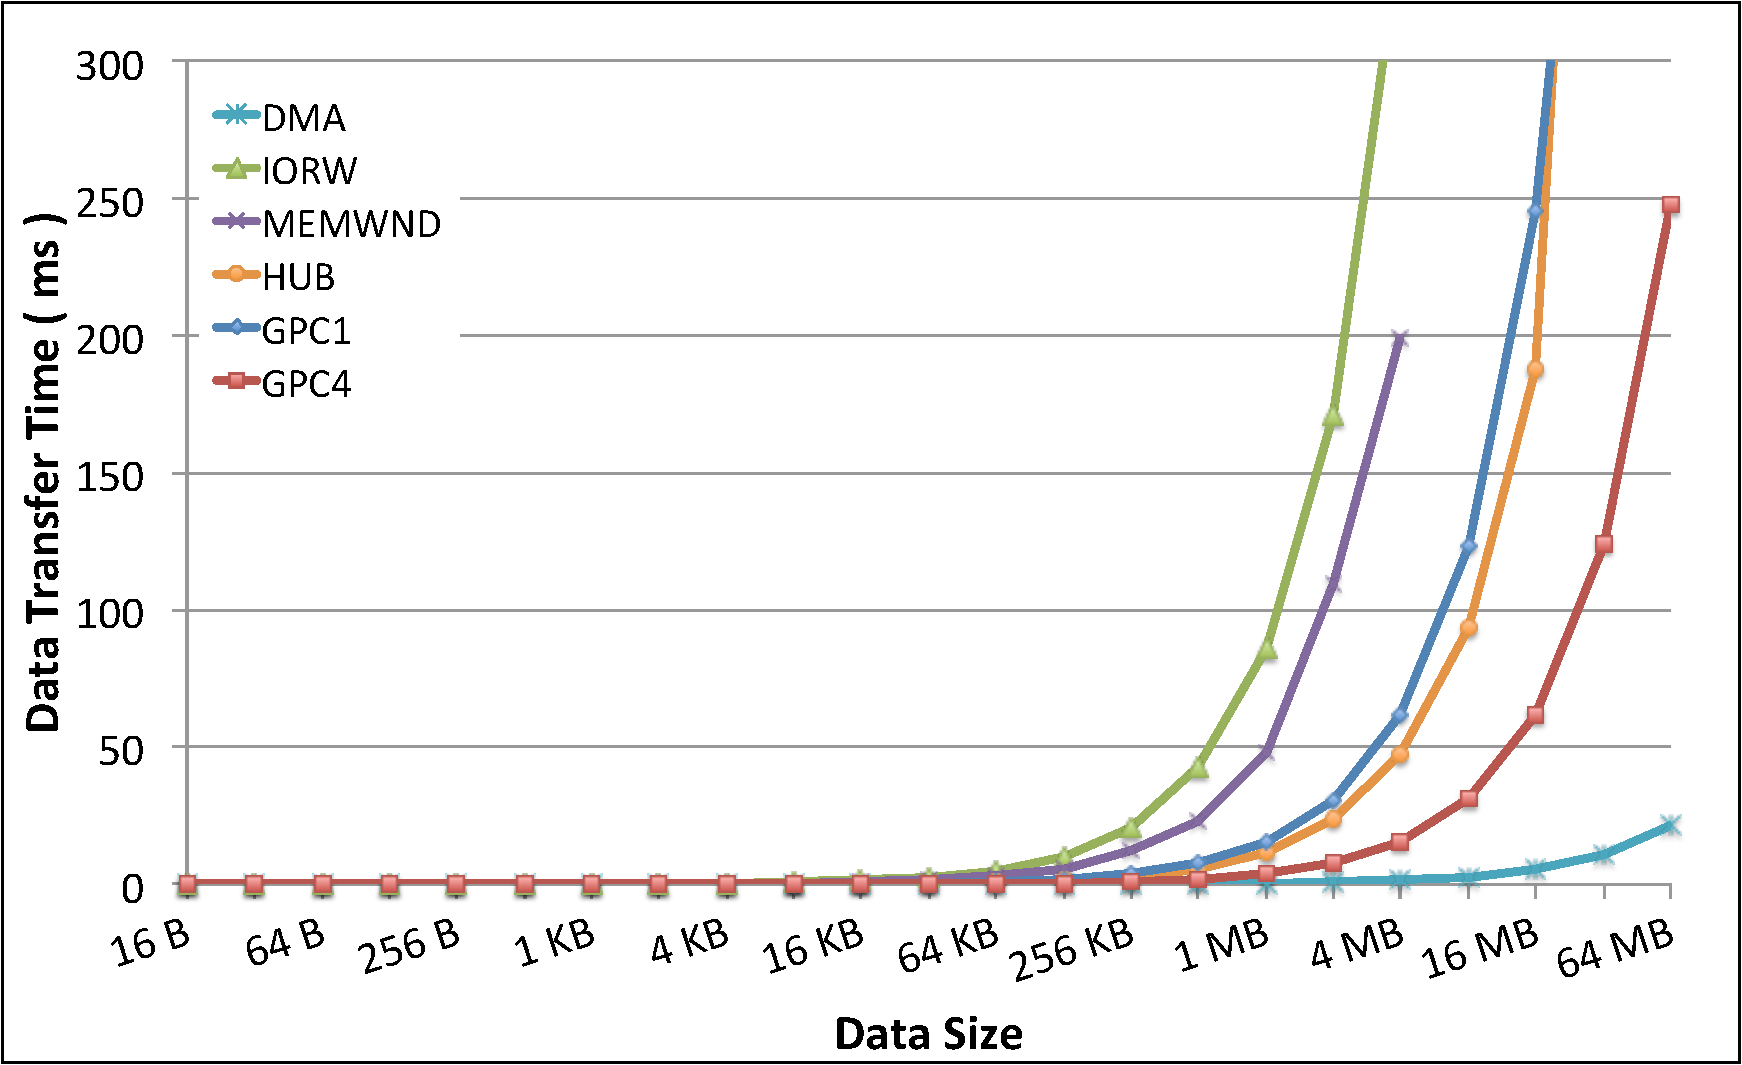
\includegraphics[width=0.34\textwidth]{figure/Graph/realtask/Memcpy_rtask_hackbench_DtoH_worst.pdf}}
  \caption{Worst-case performance of each data transfer method with a
  real-time task in the presence of \textsf{hackbench}.}
  \label{fig:worst_realtime_hackbench}
 \end{center}
\end{figure}

Figure~\ref{fig:average_realtime_hackbench}~and~\ref{fig:worst_realtime_hackbench}
show the average and the worst-case performance of each data transfer
method respectively, when a misbehaving \textsf{hackbench} process is running.
\textsf{hackbench} is a tool that generates many processes executing I/O
system calls with pipes.

\begin{figure}[!t]
 \centering
 \subfigure[Host to Device]{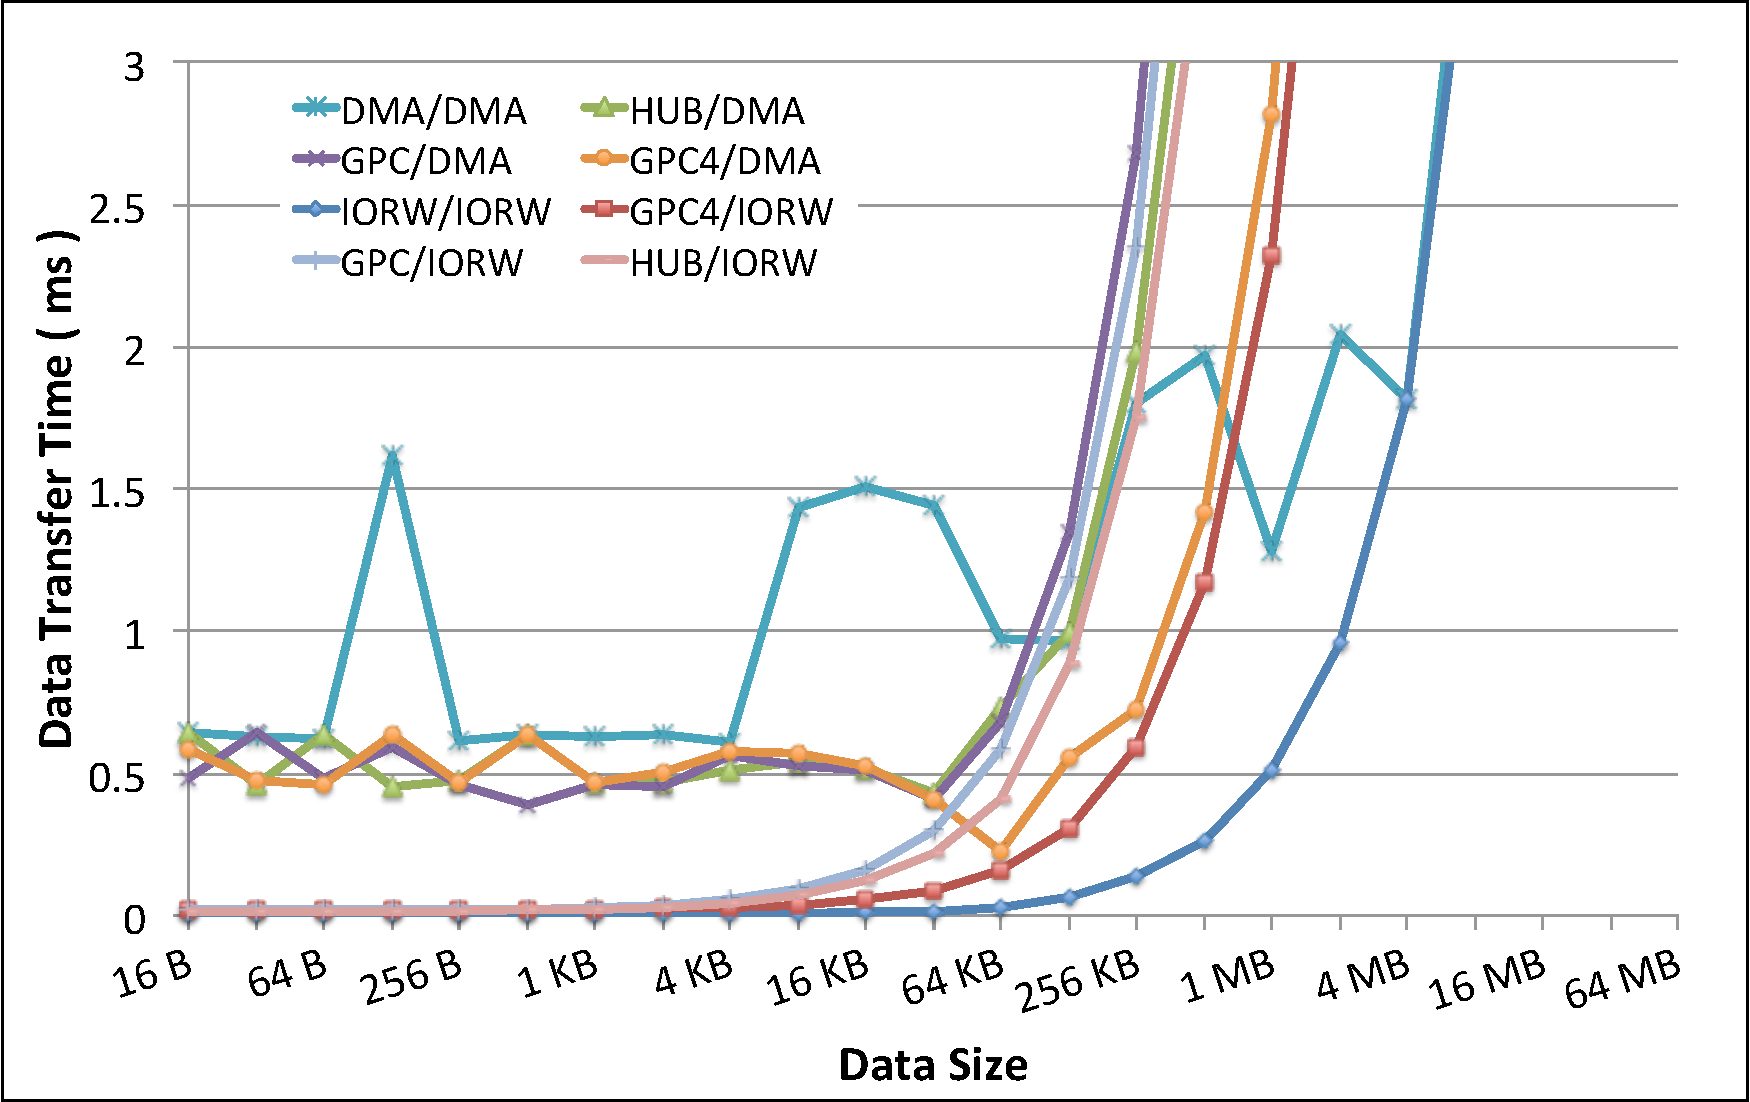
\includegraphics[width=0.34\textwidth]{figure/Graph/not_realtask/Memcpy_hybrid_HtoD.pdf}}\\
 \subfigure[Device to Host]{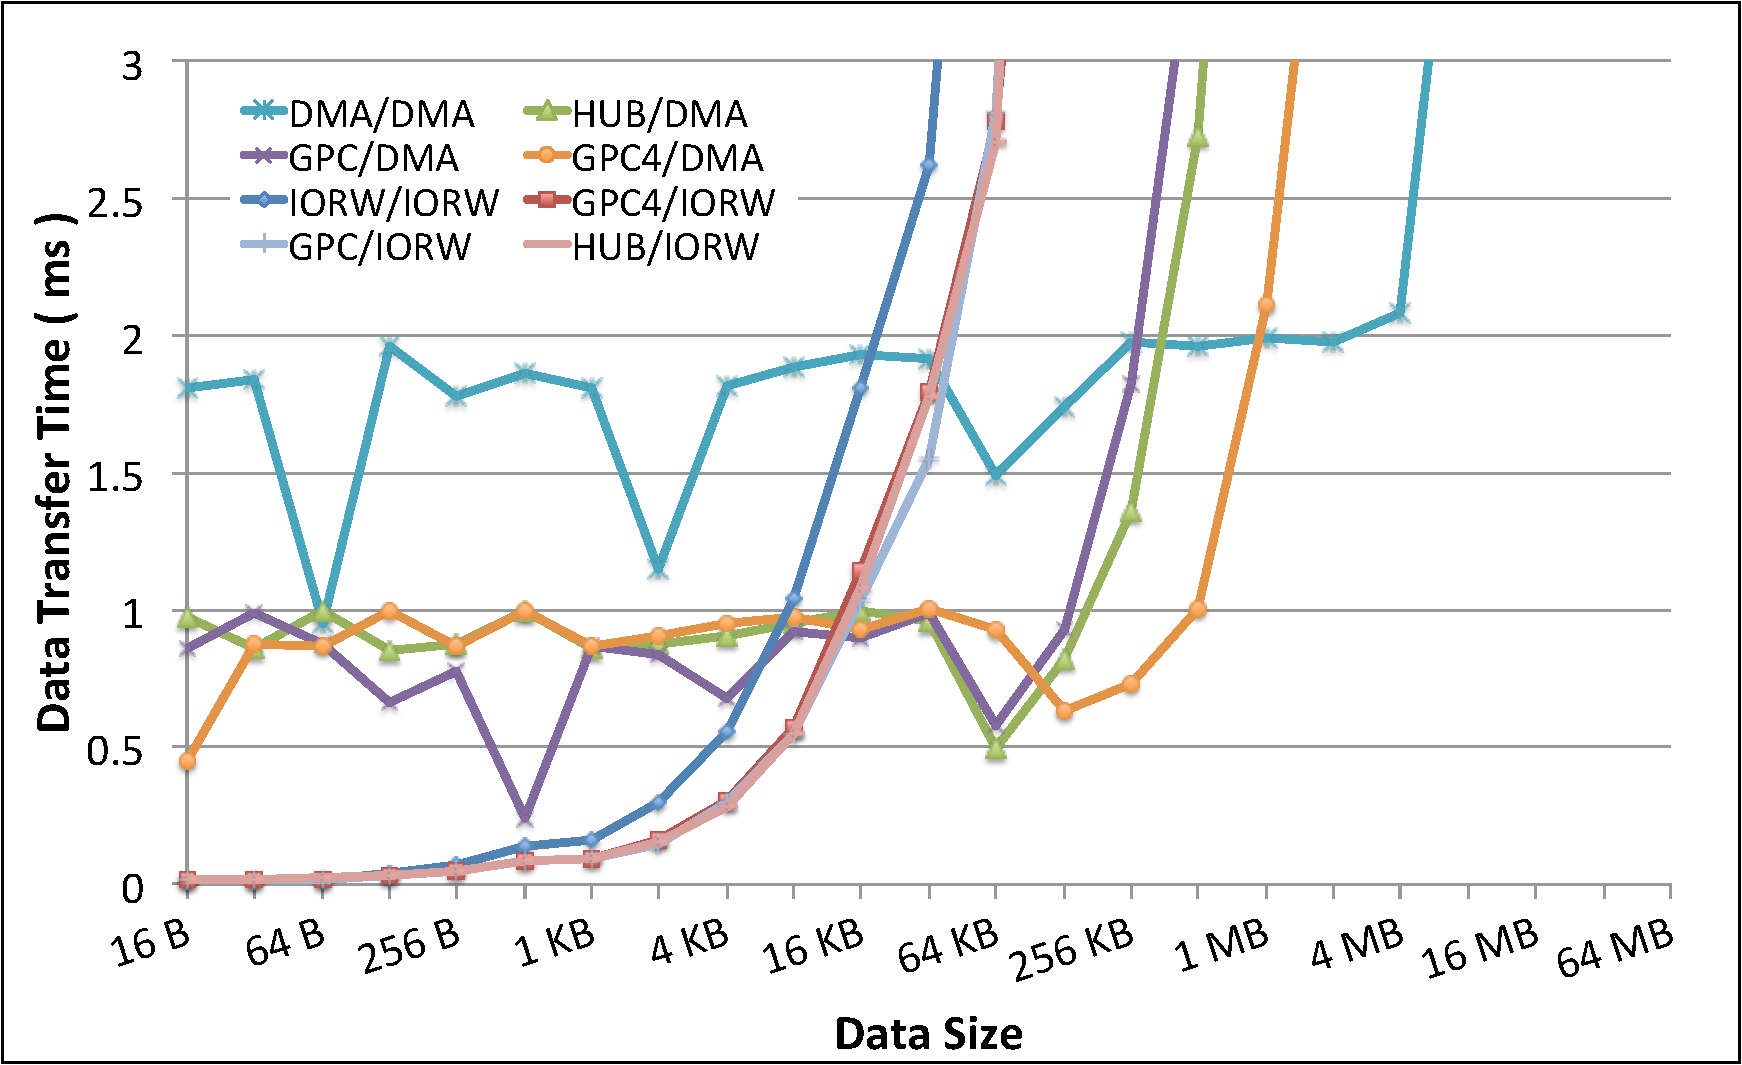
\includegraphics[width=0.34\textwidth]{figure/Graph/not_realtask/Memcpy_hybrid_DtoH.pdf}}\\
 \caption{Average performance of of concurrent two streams.}
 \label{fig:average_data_transfer_concurrent}
\end{figure}

\begin{comment}
\begin{figure}[!t]
 \centering
 \subfigure[Host to Device]{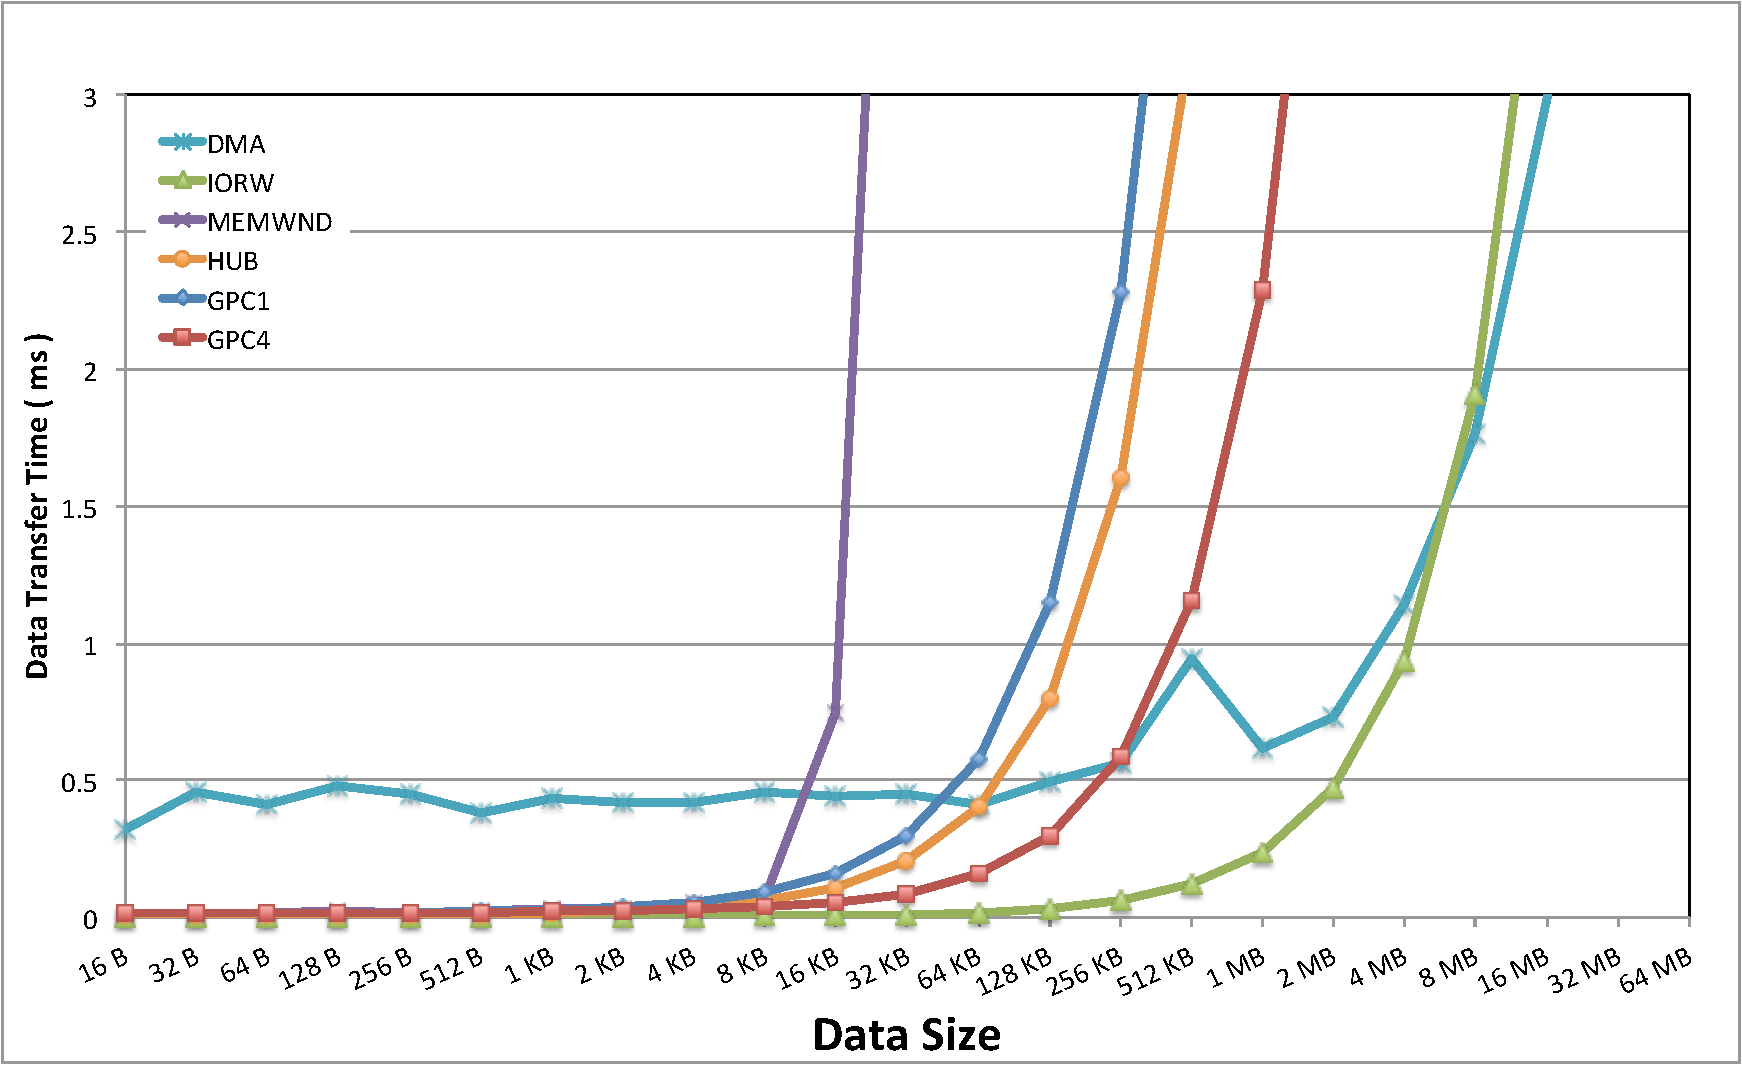
\includegraphics[width=0.4\textwidth]{figure/Graph/not_realtask/Memcpy_memswap_HtoD.pdf}}\\
 \subfigure[Device to Host]{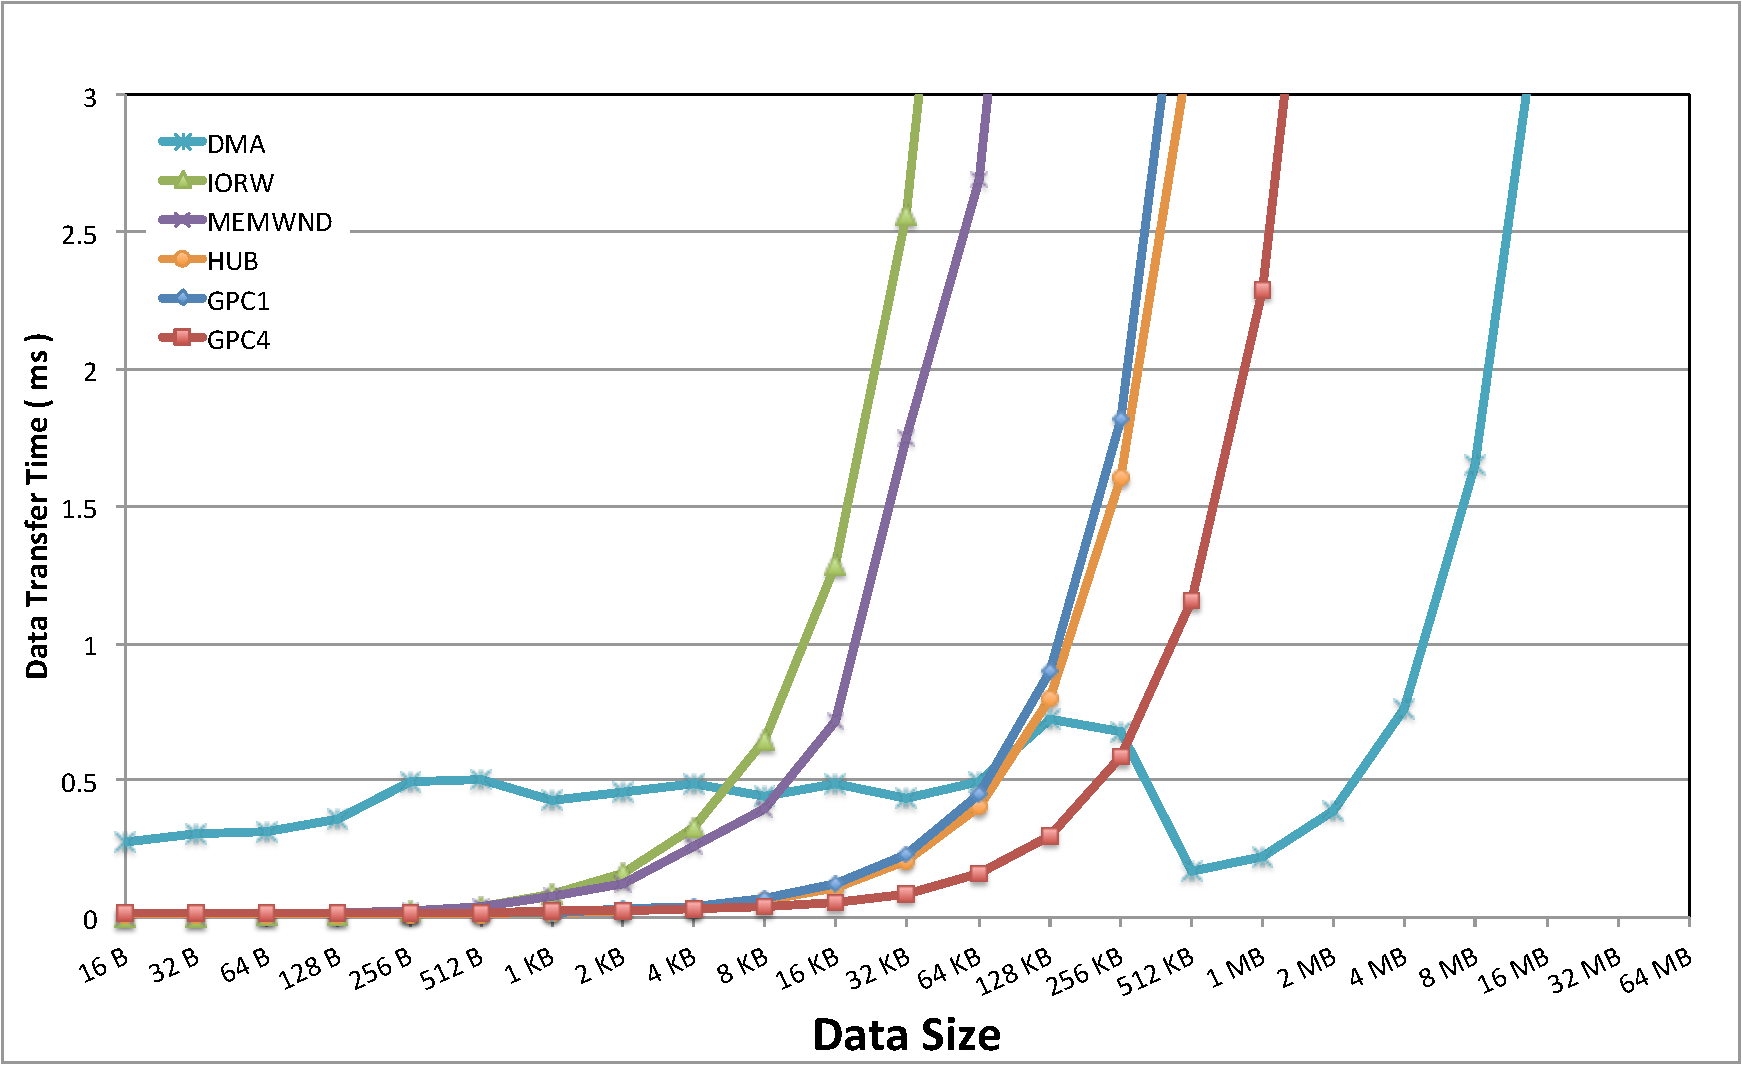
\includegraphics[width=0.4\textwidth]{figure/Graph/not_realtask/Memcpy_memswap_DtoH.pdf}}
 \caption{Average data transfer times of single streams under high
 memory access load.} 
 \label{fig:average_data_transfer_memswap}
\end{figure}

\begin{figure}[!t]
 \centering
 \subfigure[Host to Device]{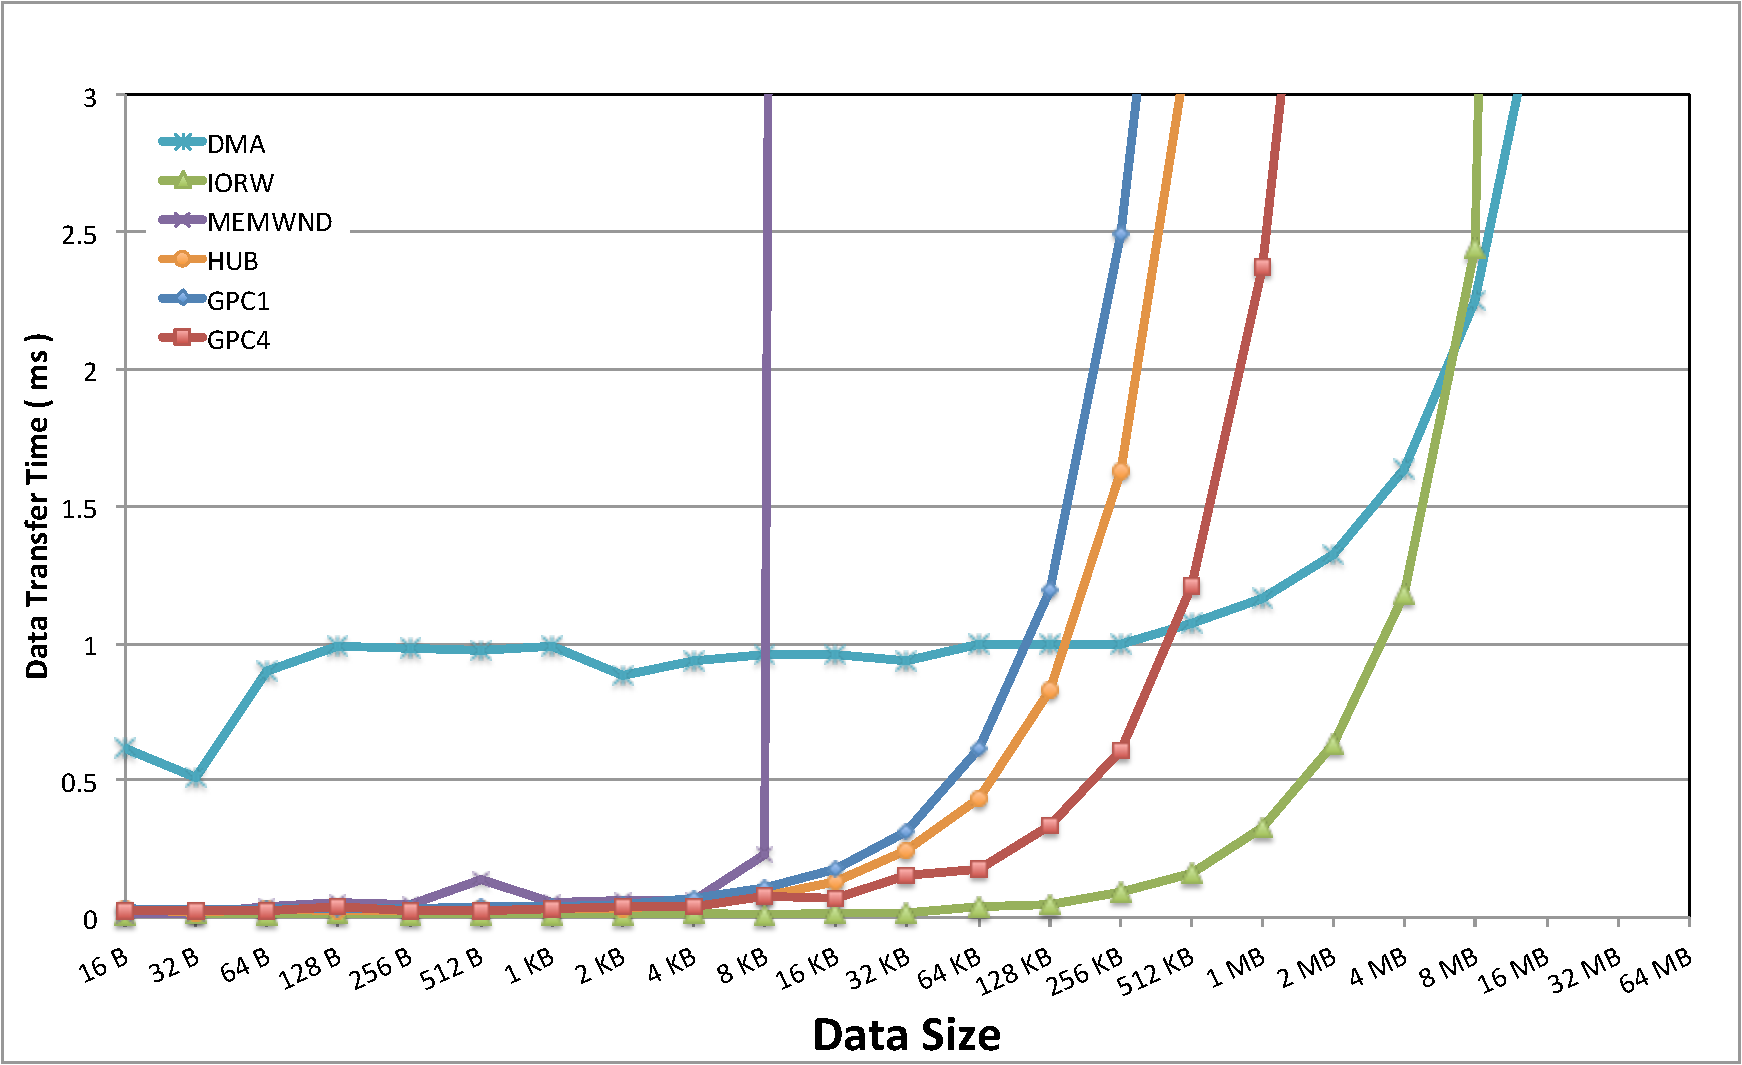
\includegraphics[width=0.4\textwidth]{figure/Graph/not_realtask/Memcpy_memswap_HtoD_worst.pdf}}\\
 \subfigure[Device to Host]{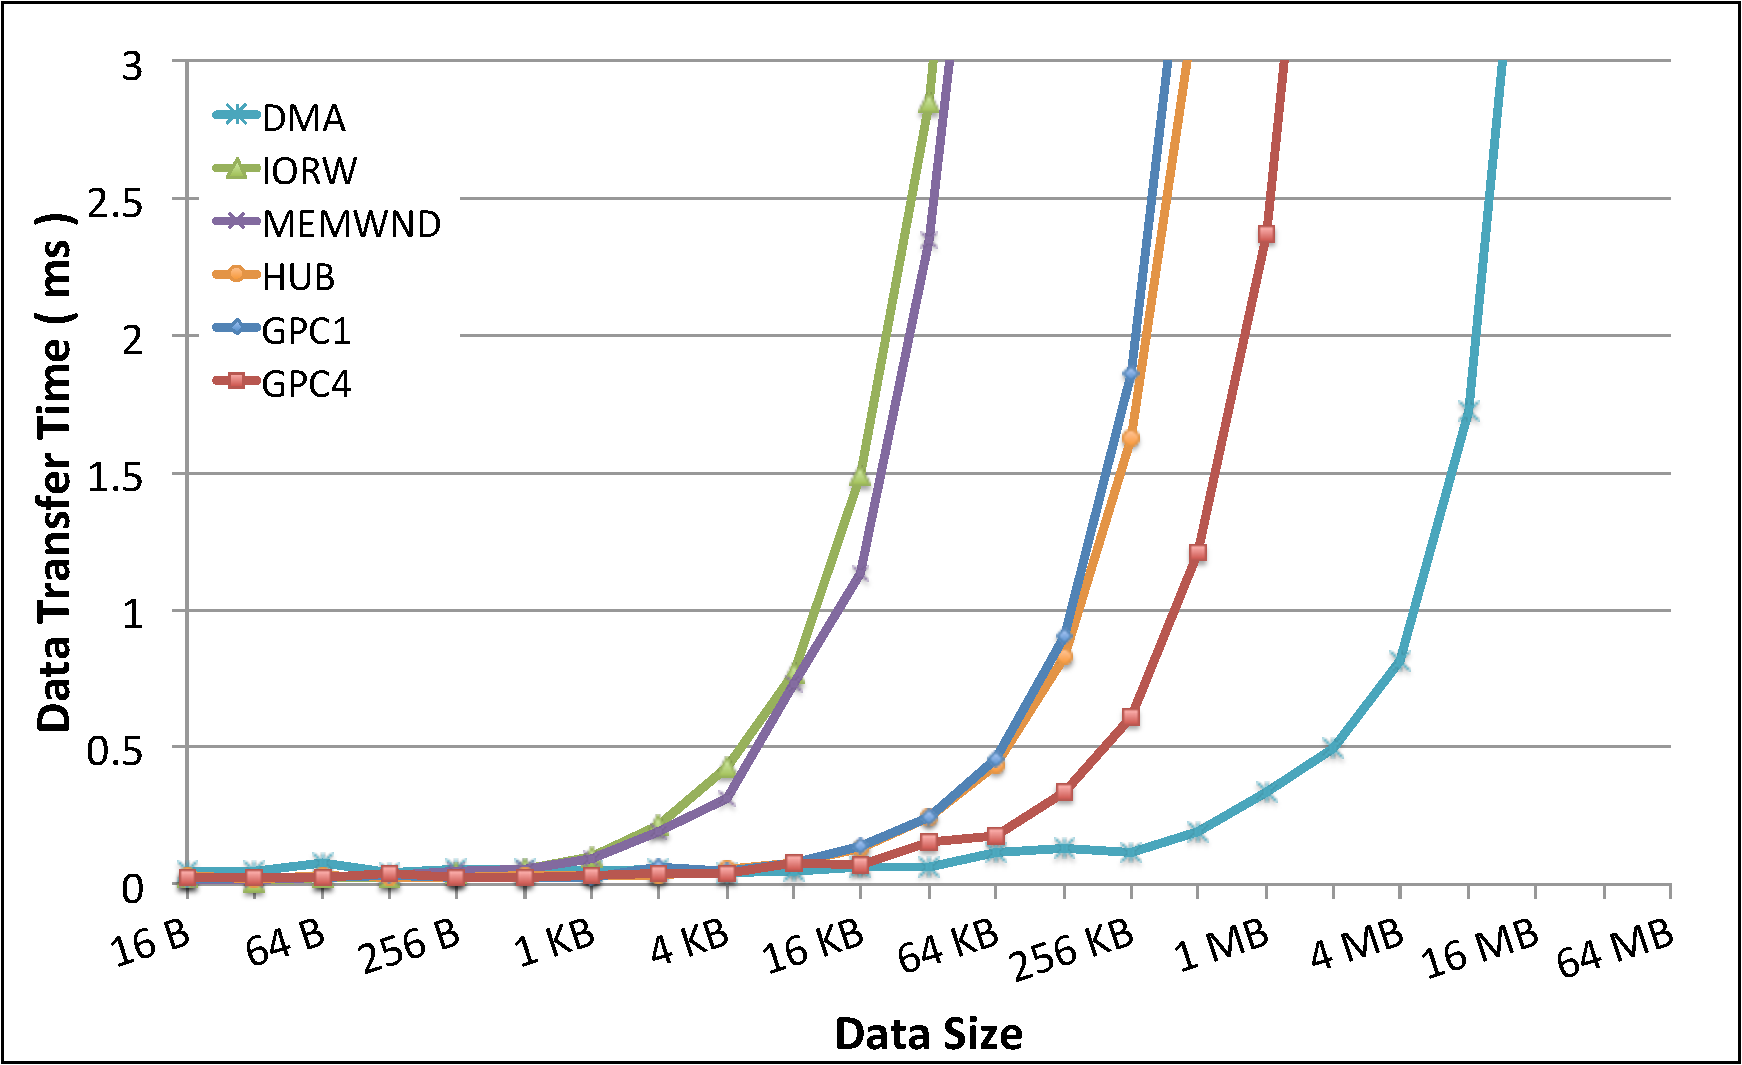
\includegraphics[width=0.4\textwidth]{figure/Graph/not_realtask/Memcpy_memswap_DtoH_worst.pdf}}
 \caption{Worst-case data transfer times of single streams under high
 memory access load.}
 \label{fig:worst_case_data_transfer_memswap}
\end{figure}

\begin{figure}[!t]
 \centering
 \subfigure[Host to Device]{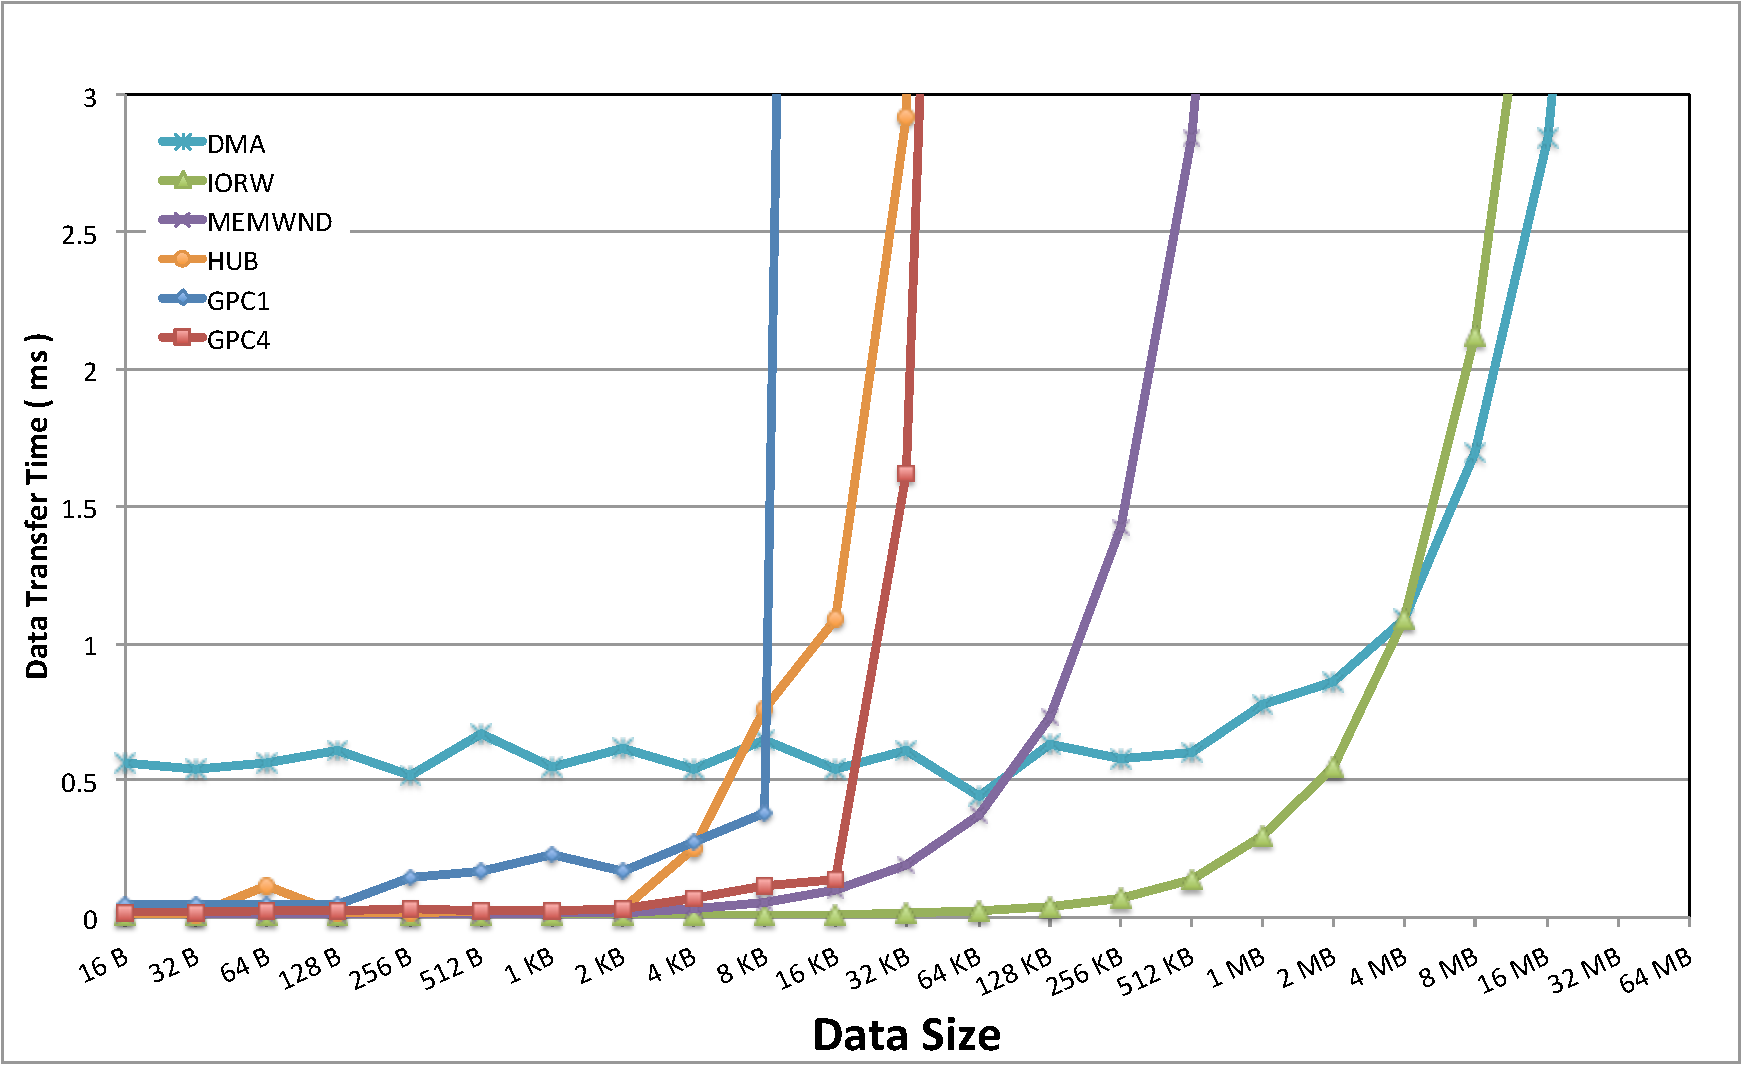
\includegraphics[width=0.4\textwidth]{figure/Graph/not_realtask/Memcpy_hackbench_HtoD.pdf}}\\
 \subfigure[Device to Host]{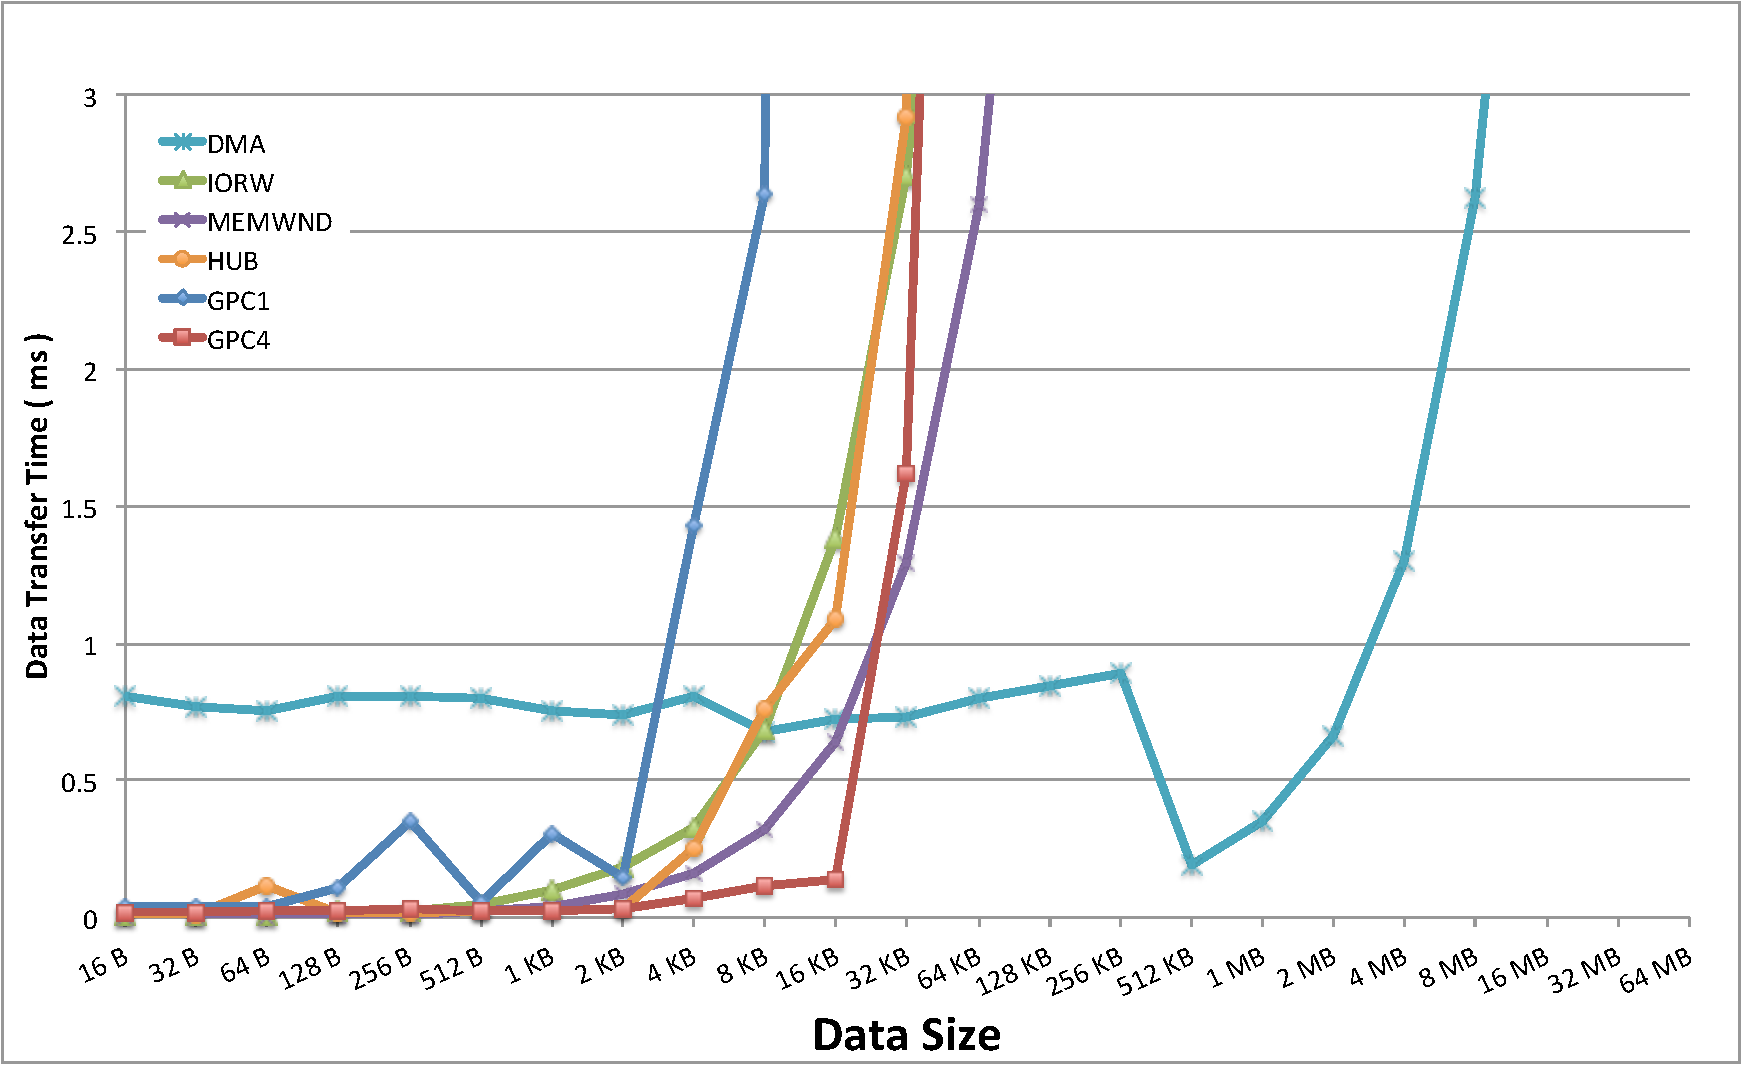
\includegraphics[width=0.4\textwidth]{figure/Graph/not_realtask/Memcpy_hackbench_DtoH.pdf}}
 \caption{Average data transfer times of single streams in the presence
 of \textsf{hackbench}.}
 \label{fig:average_data_transfer_hackbench}
\end{figure}

\begin{figure}[!t]
 \centering
 \subfigure[Host to Device]{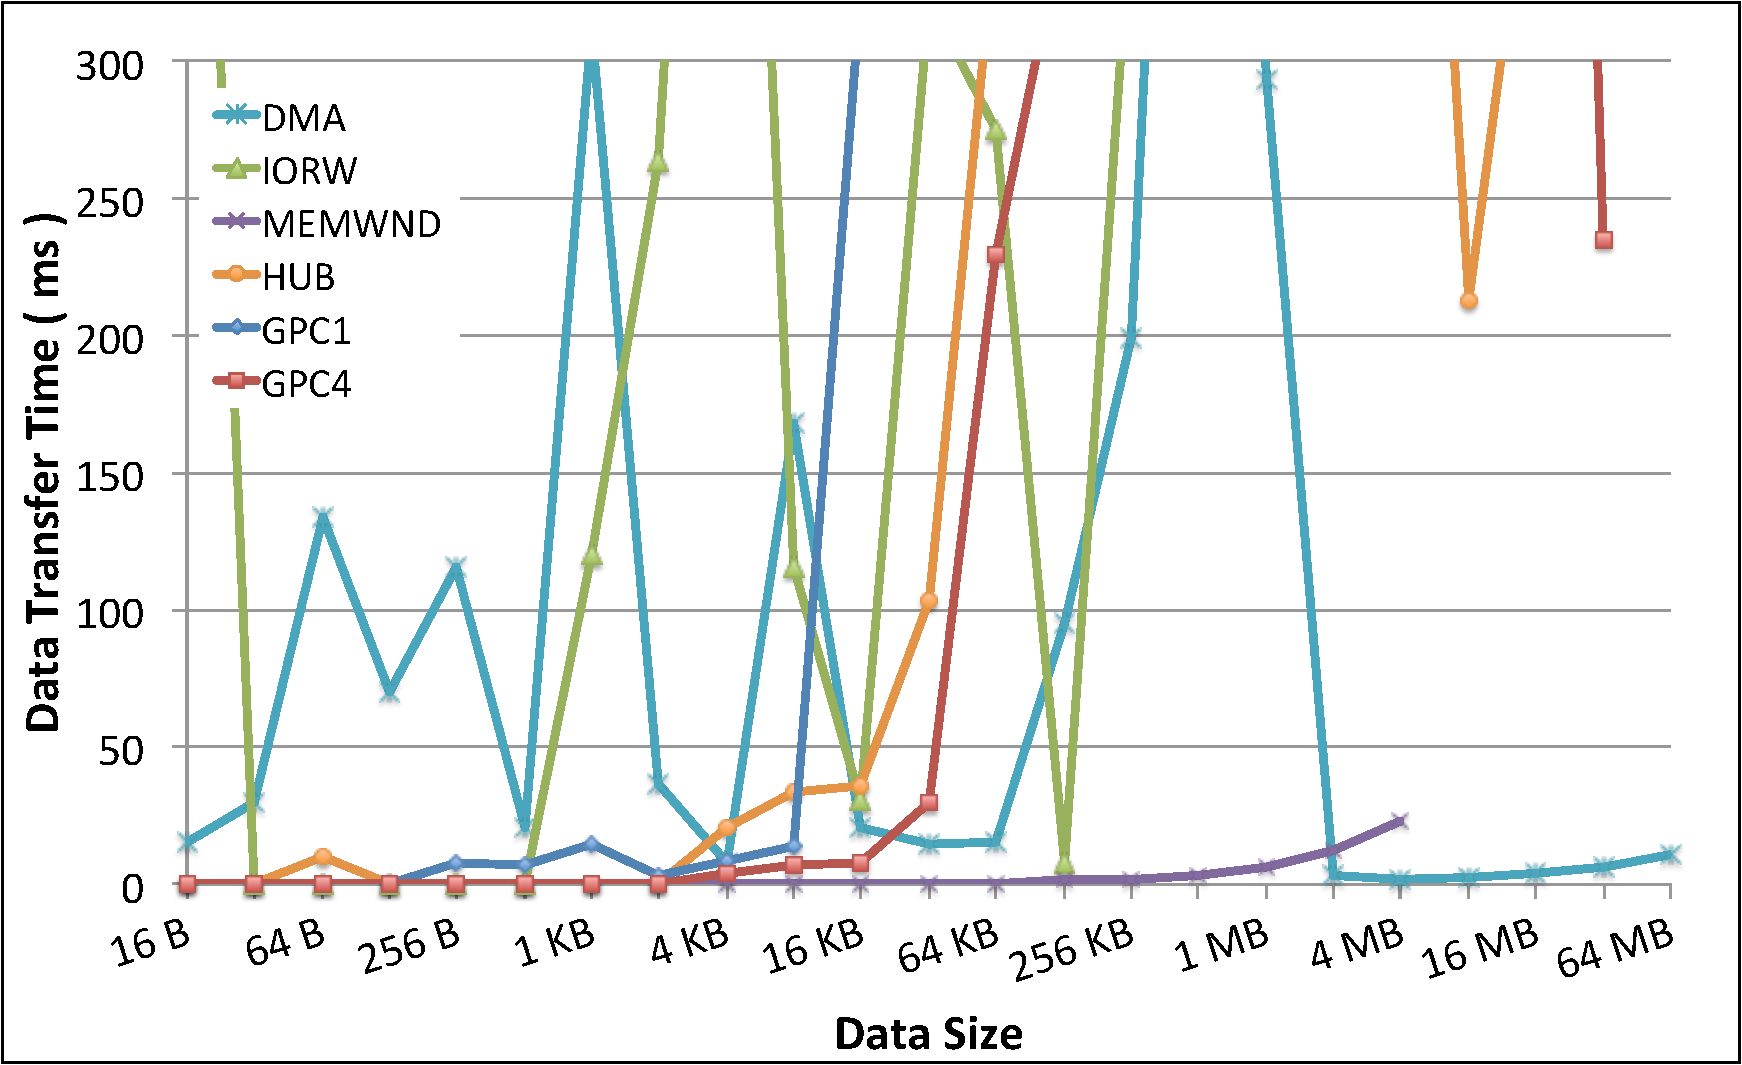
\includegraphics[width=0.4\textwidth]{figure/Graph/not_realtask/Memcpy_hackbench_HtoD_worst.pdf}}\\
 \subfigure[Device to Host]{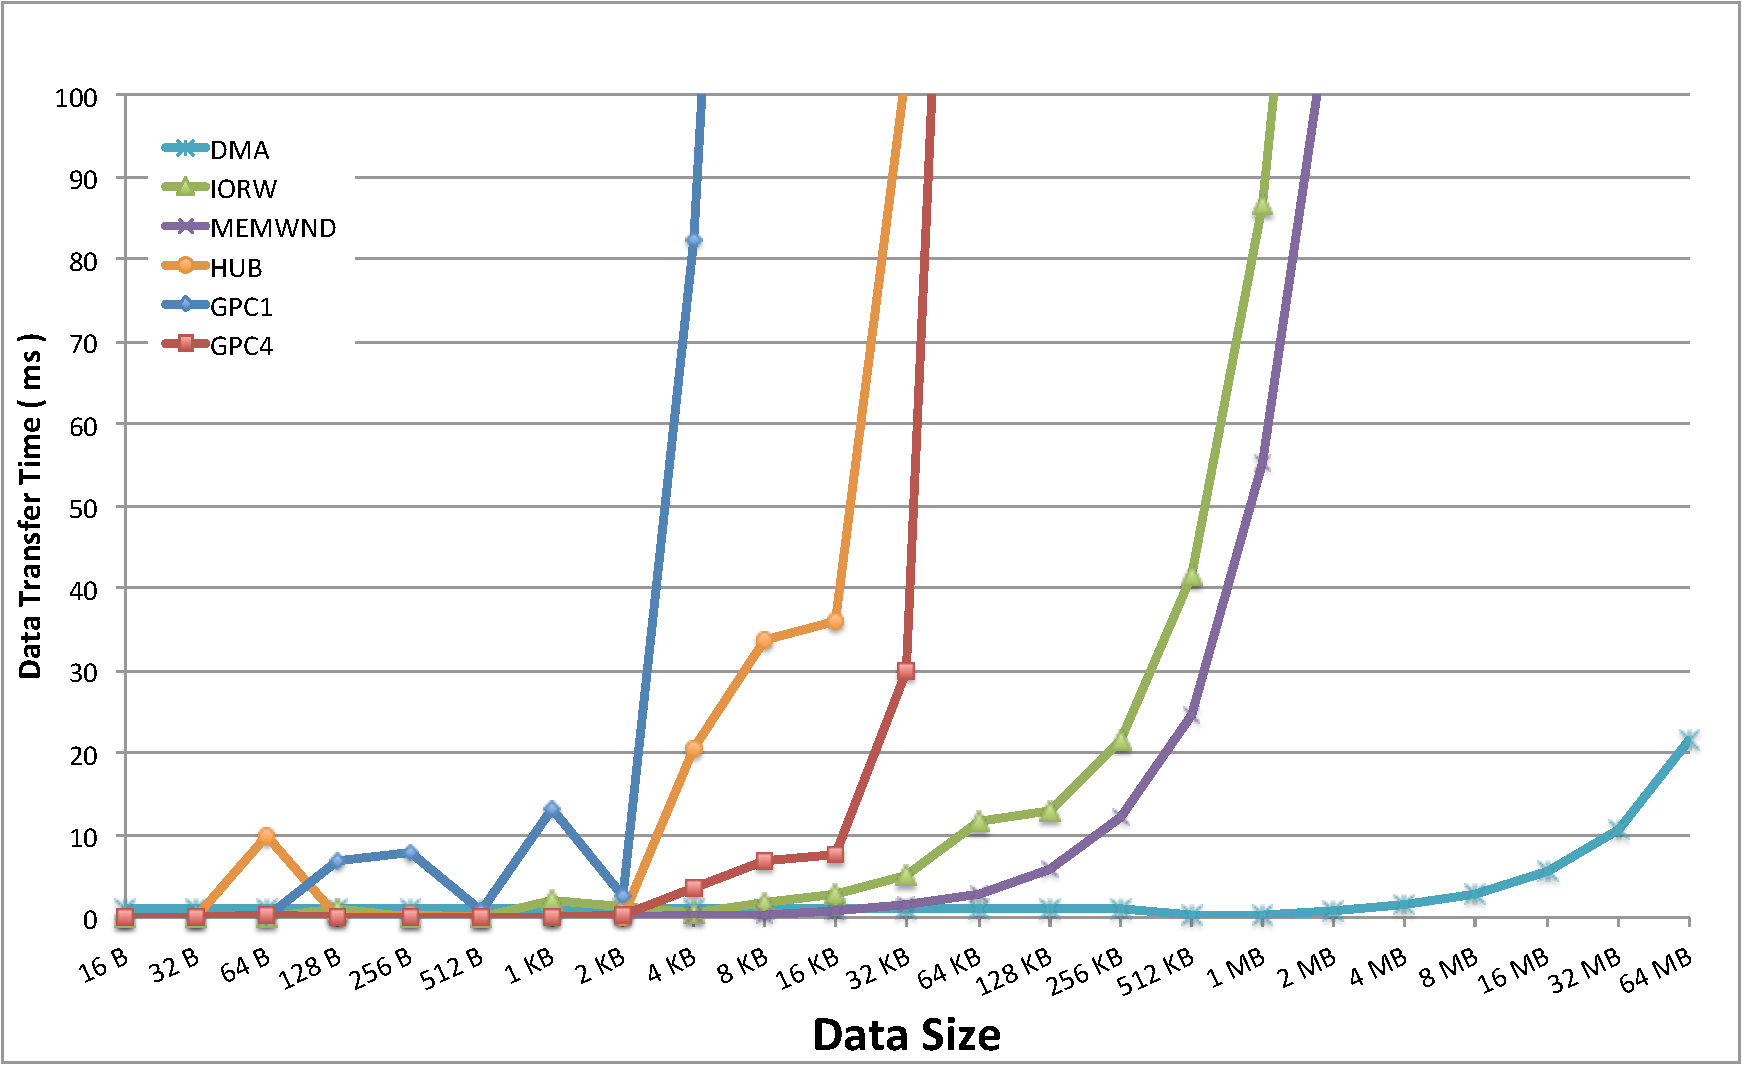
\includegraphics[width=0.4\textwidth]{figure/Graph/not_realtask/Memcpy_hackbench_DtoH_worst.pdf}}
 \caption{Worst-case data transfer times of single streams in the
 presence of \textsf{hackbench}.}
 \label{fig:worst_case_data_transfer_hackbench}
\end{figure}
\end{comment}